\newpage
\section{TÍCH VÔ HƯỚNG CỦA HAI VÉC-TƠ}
\subsection{LÝ THUYẾT CẦN NHỚ}
\subsubsection{Góc giữa hai véc-tơ}
\iconMT \indam{Định nghĩa:}
	\begin{boxdn}
	 Cho hai véc-tơ $\overrightarrow{a}$ và $\overrightarrow{b}$ đều khác $\overrightarrow{0}$. Từ một điểm $O$ bất kì ta vẽ $\overrightarrow{O A}=\overrightarrow{a}$, $\overrightarrow{O B}=\overrightarrow{b}$. \\
	 Góc $\widehat{A O B}$ với số đo từ $0^{\circ}$ đến $180^{\circ}$ được gọi là góc giữa hai véc-tơ $\overrightarrow{a}$ và $\overrightarrow{b}$. \\
	 Ta kí hiệu góc giữa hai véc-tơ $\overrightarrow{a}$ và $\overrightarrow{b}$ là $\left (\overrightarrow{a}, \overrightarrow{b} \right )$. \\
	 \begin{center}
	 	\begin{tikzpicture}[scale=1, font=\footnotesize, line join=round, line cap=round,>=stealth]
	 		\path
	 		(4,3) coordinate (A) 
	 		(5,1) coordinate (B) 
	 		(0,3) coordinate (C) 
	 		(2,2) coordinate (D)
	 		(0,1) coordinate (E)
	 		(1,2) coordinate (F)
	 		(3,2) coordinate (O)
	 		;
	 		\path  pic[draw,angle radius=8] {angle=B--O--A}  ;
	 		\draw[->,red] (O)--(B); \draw[->,red] (C)--(D); 
	 		\draw[->,cyan] (O)--(A); \draw[->,cyan] (E)--(F); 
	 		\draw (2.5,1)  node[below=0.3cm]{\text{Hình 2}} ;
	 		\draw ($(C)!0.5!(D)$) node[above]{$\overrightarrow{a}$}   ($(O)!0.5!(A)$) node[above]{$\overrightarrow{b}$}
	 		($(E)!0.5!(F)$) node[above]{$\overrightarrow{b}$} ($(O)!0.5!(B)$) node[below]{$\overrightarrow{a}$};
	 		\foreach \x/\g in {A/90,B/90,O/180} 
	 		\fill[black] (\x)  +(\g:3mm) node {$\x$};
	 	\end{tikzpicture}
	 \end{center}
	 Nếu $\left (\overrightarrow{a}, \overrightarrow{b} \right )=90^{\circ}$ thì ta nói rằng $\overrightarrow{a}$ và $\overrightarrow{b}$ vuông góc với nhau, kí hiệu là $\overrightarrow{a} \perp \overrightarrow{b}$.
	\end{boxdn}
	
\begin{khung4}{Lưu ý}
		\begin{itemize}
			\item Từ định nghĩa ta có $\left (\overrightarrow{a}, \overrightarrow{b}\right )=\left (\overrightarrow{b}, \overrightarrow{a}\right )$.
			\item Góc giữa hai véc-tơ cùng hướng và khác $\overrightarrow{0}$ luôn bằng $0^{\circ}$.
			\item Góc giữa hai véc-tơ ngược hướng và khác $\overrightarrow{0}$ luôn bằng $180^{\circ}$.
			\item Trong trường hợp có ít nhất một trong hai véc-tơ $\overrightarrow{a}$ hoặc $\overrightarrow{b}$ là véc-tơ $\overrightarrow{0}$ thì ta quy ước số đo góc giữa hai véc-tơ đó là tuỳ ý (từ $0^{\circ}$ đến $180^{\circ}$).
		\end{itemize}
		\begin{center}
			\begin{tikzpicture}[scale=1, font=\footnotesize, line join=round, line cap=round,>=stealth]
				\path
				(0,0) coordinate (A) 
				(2,0) coordinate (B) 
				(3.5,0) coordinate (C) 
				(5,0) coordinate (D)
				(7.5,0) coordinate (E)
				(9,0) coordinate (F)
				;
				\draw[->,red] (A)--(B); \draw[->,red] (E)--(F); 
				\draw[->,cyan] (B)--(C); \draw[->,cyan] (E)--(D); 
				\draw (5,-1)  node[below=0.3cm]{\text{Hình 3}} ;
				\draw[fill=black] ($(A)!0.5!(B)$) node[above]{$\overrightarrow{a}$}   ($(B)!0.5!(C)$) node[above]{$\overrightarrow{b}$}
				($(D)!0.5!(E)$) node[above]{$\overrightarrow{c}$} ($(E)!0.5!(F)$) node[above]{$\overrightarrow{d}$}
				($(A)!0.5!(C)$) node[below=8pt]{$\left (\overrightarrow{a},\overrightarrow{b} \right ) = 0^\circ$}
				($(D)!0.5!(F)$) node[below=8pt]{$\left (\overrightarrow{c},\overrightarrow{d} \right ) = 180^\circ$}
				(A) circle(1.1pt)  (E) circle(1.1pt);
			\end{tikzpicture}
		\end{center}
\end{khung4}


\subsubsection{Tích vô hướng của hai véc-tơ}
\iconMT \indam{Định nghĩa:}
\begin{boxdn}
	Cho hai véc-tơ $\overrightarrow{a}$ và $\overrightarrow{b}$ đều khác $\overrightarrow{0}$. \\
	Tích vô hướng của $\overrightarrow{a}$ và $\overrightarrow{b}$ là một số, kí hiệu là $\overrightarrow{a} \cdot \overrightarrow{b}$, được xác định bởi công thức:
	$$
	\overrightarrow{a} \cdot \overrightarrow{b}=\left |\overrightarrow{a} \right | \cdot \left |\overrightarrow{b} \right | \cdot \cos \left (\overrightarrow{a}, \overrightarrow{b}\right ) .
	$$
\end{boxdn}

\begin{khung4}{Lưu ý}
	\begin{itemize}
		\item    Trường hợp ít nhất một trong hai véc-tơ $\overrightarrow{a}$ và $\overrightarrow{b}$ bằng $\overrightarrow{0}$, ta quy ước $\overrightarrow{a} \cdot \overrightarrow{b}=0$.
		\item    Với $\overrightarrow{a}$ và $\overrightarrow{b}$ đều khác $\overrightarrow{0}$, ta có $\overrightarrow{a} \perp \overrightarrow{b} \Leftrightarrow \overrightarrow{a} \cdot \overrightarrow{b}=0$.
		\item    Khi $\overrightarrow{a}=\overrightarrow{b}$ thì tích vô hướng $\overrightarrow{a} \cdot \overrightarrow{b}$ được kí hiệu là $\overrightarrow{a}^{2}$ và được gọi là bình phuơng vô hướng của véc-tơ $\overrightarrow{a}$.
		\item Ta có $\overrightarrow{a}^{2}=|\overrightarrow{a}| \cdot|\overrightarrow{a}| \cdot \cos 0^{\circ}=|\overrightarrow{a}|^{2}$. Vậy bình phương vô hướng của một véc-tơ luôn bằng bình phương độ dài của véc-tơ đó.
		\item Trong Vật lí, tích vô hướng của $\overrightarrow{F}$ và $\overrightarrow{d}$ biểu diễn công $A$ sinh bởi lực $\overrightarrow{F}$ khi thực hiện độ dịch chuyển $\overrightarrow{d}$. Ta có công thức: $A=\overrightarrow{F} \cdot  \overrightarrow{d}$.
	\end{itemize}
\end{khung4}

\subsubsection{Tính chất của tích vô hướng}
\iconMT \indam{Tính chất:}
\begin{boxdn}
	Với ba véc-tơ $\overrightarrow{a}$, $\overrightarrow{b}$, $\overrightarrow{c}$ bất kì và mọi số $k$, ta có
	\begin{itemize}
		\item   $\overrightarrow{a} \cdot \overrightarrow{b}=\overrightarrow{b} \cdot \overrightarrow{a}$;
		\item   $\overrightarrow{a} \cdot \left (\overrightarrow{b}+\overrightarrow{c}\right )=\overrightarrow{a} \cdot \overrightarrow{b}+\overrightarrow{a} \cdot \overrightarrow{c}$;
		\item   $\left (k \overrightarrow{a}\right ) \cdot \overrightarrow{b}=k\left (\overrightarrow{a} \cdot \overrightarrow{b}\right )=\overrightarrow{a} \cdot \left (k \overrightarrow{b} \right )$.
	\end{itemize}
\end{boxdn}

\begin{khung4}{Lưu ý}
	\begin{itemize}
		\item $\left (\overrightarrow{a}+\overrightarrow{b} \right )^{2}=\overrightarrow{a}^{2}+2 \overrightarrow{a} \cdot \overrightarrow{b}+\overrightarrow{b}^{2}$.
		\item $\left (\overrightarrow{a}-\overrightarrow{b} \right )^{2}=\overrightarrow{a}^{2}-2 \overrightarrow{a} \cdot \overrightarrow{b}+\overrightarrow{b}^{2}$.
		\item  $\left (\overrightarrow{a}+\overrightarrow{b} \right ) \cdot \left (\overrightarrow{a}-\overrightarrow{b} \right )=\overrightarrow{a}^{2}-\overrightarrow{b}^{2}$.
	\end{itemize}
\end{khung4}

%-------------------------------------------------------------------------------------------------------------
\subsection{PHÂN LOẠI VÀ PHƯƠNG PHÁP GIẢI TOÁN}
\begin{dang}{Tính tích vô hướng của hai véc-tơ và xác định góc}
\end{dang}

\begin{vd}%[0H5H4-1]%[Dự án đề cương 3 Khối NH24-25-Dot 1-Nguyễn Hoài Nam]
	Cho tam giác $ ABC $ vuông tại $ A $ và có $ \widehat{B}=50^\circ $. Hãy tính các góc $ \left( \overrightarrow{BA},\overrightarrow{BC} \right) $; $ \left( \overrightarrow{AB},\overrightarrow{BC} \right) $; $ \left( \overrightarrow{CA},\overrightarrow{CB} \right) $; $ \left( \overrightarrow{AC},\overrightarrow{BC} \right) $; $ \left( \overrightarrow{AC},\overrightarrow{CB} \right) $; $ \left( \overrightarrow{AC},\overrightarrow{BA} \right) $.
	\loigiai{
		Vẽ điểm $ D $ sao cho $ ABDC $ là hình chữ nhật và vẽ điểm $ E $ sao cho $ B $ là trung điểm của $ AE $.
		\immini{
			\begin{itemize}
				\item $ \left( \overrightarrow{BA},\overrightarrow{BC} \right)=\widehat{ABC}=50^\circ $.
				\item $ \left( \overrightarrow{AB},\overrightarrow{BC} \right)=\left( \overrightarrow{BE},\overrightarrow{BC} \right)=\widehat{CBE}=130^\circ $.
				\item $ \left( \overrightarrow{CA},\overrightarrow{CB} \right)=\widehat{ACB}=40^\circ $.
				\item $ \left( \overrightarrow{AC},\overrightarrow{BC} \right)=\left( \overrightarrow{BD},\overrightarrow{BC} \right)=\widehat{DBC}=40^\circ $.
				\item $ \left( \overrightarrow{AC},\overrightarrow{CB} \right)=180^\circ-\left( \overrightarrow{AC},\overrightarrow{BC} \right)=180^\circ -40^\circ=140^\circ $
				\item $ \left( \overrightarrow{AC},\overrightarrow{BA} \right)=\left( \overrightarrow{BD},\overrightarrow{BA} \right)=\widehat{ABD}=90^\circ $
			\end{itemize}
		}{
		\begin{tikzpicture}[scale=1, font=\footnotesize, line join=round, line cap=round, >=stealth]
			% Toạ độ các điểm
			\coordinate (A) at (0,0);
			\coordinate (B) at (3,0);
			\coordinate (C) at (0,4);
			\coordinate (D) at (3,4);
			\coordinate (E) at (6,0);
			
			% Các đoạn thẳng
			\draw (A) -- (C) -- (B) -- (D);
			\draw (A) -- (B) -- (E);
			
			% Đánh dấu góc
			\draw pic["$50^\circ$", draw=black, angle radius=12, angle eccentricity=1.4] {angle=C--B--A};
			
			% Đánh dấu độ dài bằng nhau
			%\draw[thick, violet] ($(A)!0.5!(C)+(0.2,0)$) -- ($(A)!0.5!(C)-(0.2,0)$);
			%\draw[thick, violet] ($(B)!0.5!(D)+(0.2,0)$) -- ($(B)!0.5!(D)-(0.2,0)$);
			\draw ($(A)!0.5!(B)+(0,0.15)$) -- ($(A)!0.5!(B)-(0,0.15)$);
			\draw ($(B)!0.5!(E)+(0,0.15)$) -- ($(B)!0.5!(E)-(0,0.15)$);
			
			% Tên điểm
			\foreach \x/\g in {A/-90,B/-90,C/90,D/90,E/-90}
			\fill[black] 	(\x) circle (1pt)
			($(\g:3mm)+(\x)$) node {$\x$};
		\end{tikzpicture}
		}
	}
\end{vd}

\begin{vd}%[0H5H4-1]%[Dự án đề cương 3 Khối NH24-25-Dot 1-Nguyễn Hoài Nam]
	Cho tam giác đều $ ABC $ có cạnh $ a $ và trọng tâm $ G $. Tính các tích vô hướng $ \overrightarrow{AB}\cdot \overrightarrow{AC} $; $ \overrightarrow{AC}\cdot \overrightarrow{CB} $; $ \overrightarrow{AG}\cdot \overrightarrow{AB} $; $ \overrightarrow{GB}\cdot \overrightarrow{GC} $; $ \overrightarrow{BG}\cdot \overrightarrow{GA} $; $ \overrightarrow{GA}\cdot \overrightarrow{BC} $.
	\loigiai{
		Ta có $ G $ là trọng tâm của tam giác đều $ ABC $ nên $ GA=GB=GC=\dfrac{2}{3}\cdot \dfrac{a\sqrt{3}}{2}=\dfrac{a\sqrt{3}}{3} $.
		\immini{
			Ta có\\
			$ \overrightarrow{AB}\cdot \overrightarrow{AC}=a\cdot a\cdot \cos 60^\circ =\dfrac{1}{2}a^2 $;\\
			$ \overrightarrow{AC}\cdot \overrightarrow{CB}=a\cdot a\cdot \cos 120^\circ=-\dfrac{1}{2}a^2 $;\\
			$ \overrightarrow{AG}\cdot \overrightarrow{AB}=\dfrac{a\sqrt{3}}{3}\cdot a\cdot \cos 30^\circ=a^2\cdot \dfrac{\sqrt{3}}{2}\cdot \dfrac{\sqrt{3}}{2}=\dfrac{1}{2}a^2 $;\\
			$ \overrightarrow{GB}\cdot \overrightarrow{GC}=\dfrac{a\sqrt{3}}{3}\cdot \dfrac{a\sqrt{3}}{3}\cdot \cos 120^\circ =-\dfrac{a^2}{6} $;\\
			$ \overrightarrow{BG}\cdot \overrightarrow{GA}=\dfrac{a\sqrt{3}}{3}\cdot \dfrac{a\sqrt{3}}{3}\cdot \cos 60^\circ =\dfrac{a^2}{6} $;\\
			$ \overrightarrow{GA}\cdot \overrightarrow{BC}=0 $ do $ GA\perp BC $.\\
		}{
			\begin{tikzpicture}[scale=1.2, font=\footnotesize, line join=round, line cap=round, >=stealth]
				\coordinate (A) at (0,0);
				\coordinate (B) at (4,0); 
				\coordinate (C) at (2,3.39);
				\coordinate (G) at (2,1.13);
				
				% Vẽ tam giác
				\draw (A)--(B)--(C)--cycle (G)--(A) (G)--(B) (G)--(C);
				\foreach \x/\g in {A/180,B/0,C/90,G/45}
				\fill[black] 	(\x) circle (1pt)
				($(\g:3mm)+(\x)$) node {$\x$};
			\end{tikzpicture}
		}
		
		
	}
\end{vd}

\begin{vd}%[0H5H4-3]%[Dự án đề cương 3 Khối NH24-25-Dot 1-Nguyễn Hoài Nam]
	Cho hình vuông $ ABCD $ cạnh $ a $. $ M $ là trung điểm của $ AB $, $ G $ là trọng tâm tam giác $ ADM $. Tính giá trị của các biểu thức sau:
	\begin{enumerate}
		\item $ \left (\overrightarrow{AB}+\overrightarrow{AD}\right )\left (\overrightarrow{BD}+\overrightarrow{BC}\right ) $.
		\item $ \overrightarrow{CG}\left (\overrightarrow{CA}+\overrightarrow{DM}\right ) $.
	\end{enumerate}
	\loigiai{
		\begin{enumerate}
			\item 
			\immini{
				Theo quy tắc hình bình hành ta có $ \overrightarrow{AB}+\overrightarrow{AD}=\overrightarrow{AC} $. Do đó
				\[  \left (\overrightarrow{AB}+\overrightarrow{AD}\right )\left (\overrightarrow{BD}+\overrightarrow{BC}\right )=\overrightarrow{AC}\cdot \overrightarrow{BD}+\overrightarrow{AC}\cdot \overrightarrow{BC}=\overrightarrow{CA}\cdot \overrightarrow{CB}.  \]
				Theo định lý Py-ta-go ta có $ AC=\sqrt{a^2+a^2}=a\sqrt{2} $.\\
				Góc giữa hai véc-tơ $ \overrightarrow{CA} $ và $ \overrightarrow{CB} $ là góc $ ACB=45^\circ $.\\
				Vậy 
				\begin{align*}
				 \left (\overrightarrow{AB}+\overrightarrow{AD}\right )\left (\overrightarrow{BD}+\overrightarrow{BC}\right )&=\overrightarrow{CA}\cdot \overrightarrow{CB}\\
				 &=\big|\overrightarrow{CA} \big|\cdot \big|\overrightarrow{CB} \big|\cdot \cos \widehat{ACB}\\
				 &=a\cdot a\sqrt{2}\cos 45^\circ=a^2 .
				 \end{align*}
			}{
				\begin{tikzpicture}[scale=1.5, font=\footnotesize, line join=round, line cap=round, >=stealth]
					% Định nghĩa các đỉnh hình vuông ABCD
					\coordinate (A) at (0,0);
					\coordinate (B) at (2,0);
					\coordinate (C) at (2,2);
					\coordinate (D) at (0,2);
					
					% Trung điểm M của AB
					\coordinate (M) at (1,0);
					
					\coordinate (G) at (0.33,0.67);
					
					% Vẽ hình vuông
					\draw (A) -- (B) -- (C) -- (D) -- cycle;
					
					% Vẽ tam giác ADM
					\draw (A) -- (D) -- (M) -- cycle (B)--(D) (A)--(C)--(G);
					\foreach \x/\g in {A/-135,B/-45,C/45,G/120,D/135,M/-90}
					\fill[black] 	(\x) circle (1pt)
					($(\g:3mm)+(\x)$) node {$\x$};
				
				\end{tikzpicture}
			}
			
			
			\item 
			Vì $ G $ là trọng tâm của tam giác $ ADM $ nên theo quy tắc trọng tâm $$ \overrightarrow{CG}=\dfrac{1}{3}\left (\overrightarrow{CA}+\overrightarrow{CD}+\overrightarrow{CM}\right ).$$
			Mặt khác $$ \overrightarrow{CA}=\overrightarrow{CD}+\overrightarrow{CB} $$ và $$ \overrightarrow{CM}=\dfrac{1}{2}\left( \overrightarrow{CA}+\overrightarrow{CB} \right)=\dfrac{1}{2}\left( \overrightarrow{CD}+\overrightarrow{CB}+\overrightarrow{CB} \right)=\dfrac{1}{2}\overrightarrow{CD}+\overrightarrow{CB} ,$$
			suy ra $$ \overrightarrow{CG}=\dfrac{1}{3}\left (\overrightarrow{CA}+\overrightarrow{CD}+\overrightarrow{CM}\right )=\dfrac{1}{3}\left [\left( \overrightarrow{CD}+\overrightarrow{CB}\right) +\overrightarrow{CD}+\left( \dfrac{1}{2}\overrightarrow{CD}+\overrightarrow{CB}\right)\right ] =\dfrac{5}{6}\overrightarrow{CD}+\dfrac{2}{3}\overrightarrow{CB} .$$
			Theo quy tắc trung điểm thì $$ \overrightarrow{DM}=\dfrac{1}{2}\left( \overrightarrow{DA}+\overrightarrow{DB} \right)=\dfrac{1}{2}\left( \overrightarrow{CB}+\overrightarrow{CB}-\overrightarrow{CD} \right)=\overrightarrow{CB}-\dfrac{1}{2}\overrightarrow{CD} .$$
			Như vậy
			\begin{align*}
				\overrightarrow{CG}\cdot \left (\overrightarrow{CA}+\overrightarrow{DM}\right )&=\left( \dfrac{5}{6}\overrightarrow{CD}+\dfrac{2}{3}\overrightarrow{CB} \right)\left [\left( \overrightarrow{CD}+\overrightarrow{CB} \right)+\left( \overrightarrow{CB}-\dfrac{1}{2}\overrightarrow{CD}  \right)  \right ]\\
				&=\left( \dfrac{5}{6}\overrightarrow{CD}+\dfrac{2}{3}\overrightarrow{CB} \right)\left( \dfrac{1}{2}\overrightarrow{CD}+2\overrightarrow{CB} \right)\\
				&=\dfrac{5}{12}CD^2+6\overrightarrow{CD}\cdot \overrightarrow{CB}+ \dfrac{4}{3}CB^2=\dfrac{5}{12}a^2+\dfrac{4}{3}a^2=\dfrac{21a^2}{12}.
			\end{align*}
		\end{enumerate}
	}
\end{vd}

\begin{dang}{Chứng minh đẳng thức tích vô hướng hay độ dài}
\end{dang}
\begin{vd}%[0H5B2-2]%[Dự án đề cương 3 Khối NH24-25-Dot 1-Nguyễn Hoài Nam]
	Cho đoạn thẳng $AB$ và $I$ là trung điểm của $AB$. Chứng minh rằng với mỗi điểm $O$ ta có
	\begin{enumerate}
		\item $\overrightarrow{OI}\cdot\overrightarrow{IA}+\overrightarrow{OI}\cdot\overrightarrow{IB}=0$.
		\item $\overrightarrow{OI}\cdot\overrightarrow{AB}=\dfrac{1}{2}\left(\overrightarrow{OB}^2-\overrightarrow{OA}^2\right)$.
	\end{enumerate}
	\loigiai{ 
		\begin{enumerate}
			\item Vì $I$ là trung điểm $AB$ nên $\overrightarrow{IA}+\overrightarrow{IB}=\overrightarrow{0}$.\\
			Vậy $\overrightarrow{OI}\cdot\overrightarrow{IA}+\overrightarrow{OI}\cdot\overrightarrow{IB}=\overrightarrow{OI}\cdot\left(\overrightarrow{IA}+\overrightarrow{IB}\right)=\overrightarrow{OI}\cdot\overrightarrow{0}=0$.
			\item Vì $I$ là trung điểm $AB$ nên $2\overrightarrow{OI}=\overrightarrow{OB}+\overrightarrow{OA}\Leftrightarrow\overrightarrow{OI}=\dfrac{1}{2}\left(\overrightarrow{OB}+\overrightarrow{OA}\right)$. Do đó
			\begin{eqnarray*}
				\overrightarrow{OI}\cdot\overrightarrow{AB}
				& = & \dfrac{1}{2}\left(\overrightarrow{OB}+\overrightarrow{OA}\right)\cdot\left(\overrightarrow{OB}-\overrightarrow{OA}\right)\\
				& = & \dfrac{1}{2}\left(\overrightarrow{OB}+\overrightarrow{OA}\right)\cdot\overrightarrow{OB}+\dfrac{1}{2}\left(\overrightarrow{OB}+\overrightarrow{OA}\right)\cdot\left(-\overrightarrow{OA}\right)\\
				& = & \dfrac{1}{2}\overrightarrow{OB}\cdot\overrightarrow{OB}+\dfrac{1}{2}\overrightarrow{OA}\cdot\overrightarrow{OB}-\dfrac{1}{2}\overrightarrow{OB}\cdot\overrightarrow{OA}-\dfrac{1}{2}\overrightarrow{OA}\cdot\overrightarrow{OA}\\
				& = & \dfrac{1}{2}\left(\overrightarrow{OB}^2-\overrightarrow{OA}^2\right).
			\end{eqnarray*}
		\end{enumerate}
	}
\end{vd}
\begin{vd}%[0H5V4-3]%[Dự án đề cương 3 Khối NH24-25-Dot 1-Nguyễn Hoài Nam]
	Cho điểm $M$ thay đổi trên đường tròn tâm $O$ bán kính $R$ ngoại tiếp tam giác đều $ABC$ cho trước. Chứng minh $MA^2+MB^2+MC^2=6R^2$.
	\loigiai{ 
			Vì tam giác $ABC$ đều nên tâm $O$ của đường tròn ngoại tiếp đồng thời là trọng tâm của tam giác. \\
			Suy ra $\overrightarrow{OA}+\overrightarrow{OB}+\overrightarrow{OC}=\overrightarrow{0}$. Ta có
			\begin{eqnarray*}
				MA^2+MB^2+MC^2
				& = & \overrightarrow{MA}^2+\overrightarrow{MB}^2+\overrightarrow{MC}^2\\
				& = & \left(\overrightarrow{MO}+\overrightarrow{OA}\right)^2+\left(\overrightarrow{MO}+\overrightarrow{OB}\right)^2+\left(\overrightarrow{MO}+\overrightarrow{OC}\right)^2\\
				& = & 3MO^2+OA^2+OB^2+OC^2+2\overrightarrow{MO}\cdot\left(\overrightarrow{OA}+\overrightarrow{OB}+\overrightarrow{OC}\right)\\
				& = & 6R^2.
			\end{eqnarray*}
			
	}
\end{vd}
\begin{vd}%[0H5V4-3]%[Dự án đề cương 3 Khối NH24-25-Dot 1-Nguyễn Hoài Nam]
	Cho hình chữ nhật $ABCD$ có tâm $O$, $M$ là điểm bất kì. Chứng minh
	\begin{enumerate}
		\item $MA^2+MC^2=MB^2+MD^2$; 
		\item $\overrightarrow{MA}\cdot\overrightarrow{MC}=\overrightarrow{MB}\cdot\overrightarrow{MD}$.
	\end{enumerate}
	\loigiai{
		Ta có $ABCD$ là hình chữ nhật nên $O$ là trung điểm $AC$ và $BD$, do đó\\
		\immini
		{
			$\heva{& \overrightarrow{MA}+\overrightarrow{MC}=2\overrightarrow{MO} \\ & \overrightarrow{MB}+\overrightarrow{MD}=2\overrightarrow{MO}}\Rightarrow\heva{& MA^2+MB^2+2\overrightarrow{MA}\cdot\overrightarrow{MC}=4MO^2 \\ & MB^2+MD^2+2\overrightarrow{MB}\cdot\overrightarrow{MD}=4MO^2.}$
		}
		{
			\begin{tikzpicture}[scale=.7,font=\footnotesize, line join=round, line cap=round, >=stealth]
				\coordinate (A) at (0,0);
				\coordinate (B) at (4,0);
				\coordinate (C) at (4,2);
				\coordinate (D) at (0,2);
				\coordinate (O) at (2,1);
				
				
				\draw (A)--(B)--(C)--(D)--(A)--(C)
				(B)--(D);
				\foreach \x/\g in {A/150,B/30,C/-10,D/190,O/90} \fill[black](\x) circle (1pt) ($(\x)+(\g:3mm)$) node{$\x$};
				%\clip (-0.5,-2.5) rectangle (3.5,0.5);
			\end{tikzpicture}
		}
		\begin{enumerate}
			\item Ta có $ABCD$ là hình chữ nhật nên $\overrightarrow{BA}\perp\overrightarrow{DA}\Rightarrow\overrightarrow{BA}\cdot\overrightarrow{DA}=0$. Do đó
			\begin{eqnarray*}
				MA^2+MC^2 & = & \left(\overrightarrow{MB}+\overrightarrow{BA}\right)^2+\left(\overrightarrow{MD}+\overrightarrow{DC}\right)^2\\
				& = & \overrightarrow{MB}^2+\overrightarrow{MD}^2+\overrightarrow{BA}^2+\overrightarrow{DC}^2+2\overrightarrow{MB}\cdot
				\overrightarrow{BA}+2\overrightarrow{MD}\cdot\overrightarrow{DC}\\
				& = & MB^2+MD^2+2\overrightarrow{BA}^2+2\overrightarrow{BA}\left(\overrightarrow{MB}-\overrightarrow{MD}\right)\ (\text{vì}\ \overrightarrow{DC}=-\overrightarrow{BA}.)\\
				& = & MB^2+MD^2+2\overrightarrow{BA}\left(\overrightarrow{BA}+\overrightarrow{DB}\right)\\
				& = & MB^2+MD^2+2\overrightarrow{BA}\cdot\overrightarrow{DA}=MB^2+MD^2.
			\end{eqnarray*}
			\item Ta có $O$ là trung điểm $AC$ nên $\overrightarrow{OA}+\overrightarrow{OC}=\overrightarrow{0}$. Do đó
			\begin{eqnarray*}
				\overrightarrow{MA}\cdot\overrightarrow{MC} & = & \left(\overrightarrow{MO}+\overrightarrow{OA}\right)\left(\overrightarrow{MO}+\overrightarrow{OC}\right)\\
				& = & MO^2+\overrightarrow{MO}\left(\overrightarrow{OA}+\overrightarrow{OC}\right)-OA^2\\
				& = & MO^2-OA^2.
			\end{eqnarray*}
			Tương tự ta cũng chứng minh được $\overrightarrow{MB}\cdot\overrightarrow{MD}=MO^2-OB^2$.\\
			Mà $OA=OB$ nên ta có điều phải chứng minh.
		\end{enumerate}
	}
\end{vd}

\begin{dang}{Điều kiện vuông góc}
\end{dang}
\begin{vd}%[0H5H4-4]%[Dự án đề cương 3 Khối NH24-25-Dot 1-Nguyễn Hoài Nam]
	Cho hai véc-tơ $\overrightarrow{a}$ và $\overrightarrow{b}$ vuông góc với nhau và $\left |\overrightarrow{a} \right |=1$, $\left |\overrightarrow{b} \right |=\sqrt{2}$. Chứng minh hai véc-tơ $\left (2\overrightarrow{a}-\overrightarrow{b} \right )$ và $\left (\overrightarrow{a}+\overrightarrow{b} \right )$ vuông góc với nhau.
	\loigiai
	{
		Vì $\overrightarrow{a}\perp\overrightarrow{b}$ nên $\overrightarrow{a}\cdot\overrightarrow{b}=0$.\\
		Ta có
		\begin{eqnarray*}
			\left (2\overrightarrow{a}-\overrightarrow{b} \right )\cdot \left (\overrightarrow{a}+\overrightarrow{b} \right )&=&2\overrightarrow{a}^2+\overrightarrow{a}\cdot\overrightarrow{b}-\overrightarrow{b}^2\\&=&2\left |\overrightarrow{a} \right |^2+0+\left |\overrightarrow{b} \right |^2\\&=&2\cdot 1^2-\left (\sqrt{2} \right )^2=0.
		\end{eqnarray*}
		Vậy hai véc-tơ $\left (2\overrightarrow{a}-\overrightarrow{b} \right )$ và $\left (\overrightarrow{a}+\overrightarrow{b} \right )$ vuông góc với nhau.
	}
\end{vd}
\begin{vd}%[0H5H4-4]%[Dự án đề cương 3 Khối NH24-25-Dot 1-Nguyễn Hoài Nam]
	Cho $\triangle ABC$ vuông tại $A$ có $AB=c$, $AC=b$. Tính $\overrightarrow{BA}\cdot \overrightarrow{BC}$ theo $b$ và $c$.
	\loigiai
	{
		$\triangle ABC$ vuông tại $A\Rightarrow \overrightarrow{AB}\cdot\overrightarrow{AC}=0$.\\
		Ta có $\overrightarrow{BA}\cdot \overrightarrow{BC}=\overrightarrow{BA}\cdot\left (\overrightarrow{BA}+\overrightarrow{AC} \right )=\overrightarrow{BA}^2+\overrightarrow{BA}\cdot\overrightarrow{AC}=AB^2=c^2$.
	} 
\end{vd}
\begin{vd}%[0H5H4-4]%[Dự án đề cương 3 Khối NH24-25-Dot 1-Nguyễn Hoài Nam]
	Cho hai véc-tơ $\overrightarrow{a}$ và $\overrightarrow{b}$ thỏa mãn $\left |\overrightarrow{a} \right |=\left |\overrightarrow{b} \right |=1$ và hai véc-tơ $\overrightarrow{u}=\dfrac{2}{5}\overrightarrow{a}-3\overrightarrow{b}$ và $\overrightarrow{v}=\overrightarrow{a}+\overrightarrow{b}$ vuông góc với nhau. Xác định góc giữa hai véc-tơ $\overrightarrow{a}$ và $\overrightarrow{b}$.
	\loigiai
	{
		Ta có $\overrightarrow{u}\perp\overrightarrow{v}\Rightarrow\overrightarrow{u}\cdot\overrightarrow{v}=0\Rightarrow\left (\dfrac{2}{5}\overrightarrow{a}-3\overrightarrow{b} \right )\cdot\left (\overrightarrow{a}+\overrightarrow{b} \right )=0\Rightarrow \dfrac{2}{5}\overrightarrow{a}^2-\dfrac{13}{5}\overrightarrow{a}\overrightarrow{b}-3{\overrightarrow{b}}^2=0$. \quad (1)\\
		Vì $\left |\overrightarrow{a} \right |=\left |\overrightarrow{b} \right |=1$ nên từ (1) ta suy ra $\overrightarrow{a}\cdot\overrightarrow{b}=-1$.\\
		Khi đó ta có $$\cos\left (\overrightarrow{a},\overrightarrow{b} \right )=\dfrac{\overrightarrow{a}\cdot\overrightarrow{b}}{\left |\overrightarrow{a} \right |\cdot\left |\overrightarrow{b} \right |}=-1\Rightarrow\left (\overrightarrow{a},\overrightarrow{b} \right )=180^{\circ}.$$
	}
\end{vd}
\begin{dang}{Tập hợp điểm và chứng minh bất đẳng thức}
\end{dang}
\begin{vd}%[0H5V4-5]%[Dự án đề cương 3 Khối NH24-25-Dot 1-Nguyễn Hoài Nam]
	Cho hai điểm $A$, $B$ cố định có độ dài bằng $a$. 
	Tìm tập hợp điểm $M$ sao cho
	\begin{enumEX}{2}
		\item  $\overrightarrow{MA}\cdot \overrightarrow{MB}=\dfrac{3{{a}^{2}}}{4}$
		\item $\overrightarrow{MA}\cdot \overrightarrow{MB}=MA^2$
	\end{enumEX}
	\loigiai{
		\begin{enumerate}
			\item Gọi $I$ là trung điểm của $AB$ ta có
			$$\begin{aligned} \overrightarrow{MA}\cdot \overrightarrow{MB}=\dfrac{3a^2}{4}&\Leftrightarrow \left( \overrightarrow{MI}+\overrightarrow{IA} \right)\left( \overrightarrow{MI}+\overrightarrow{IB} \right)=\dfrac{3a^2}{4}\\
				&\Leftrightarrow M{{I}^{2}}-IA^2=\dfrac{3a^2}{4}\ (\text{Do}\  \overrightarrow{IB}=-\overrightarrow{IA})\\
				& \Leftrightarrow M{{I}^{2}}=\dfrac{a^2}{4}+\dfrac{3a^2}{4} 
				\Leftrightarrow MI=a.
			\end{aligned}$$
			Vậy tập hợp điểm $M$ là đường tròn tâm $I$ bán kính $R=a$.
			\item Ta có  $$\begin{aligned} \overrightarrow{MA}\cdot \overrightarrow{MB}=MA^2&\Leftrightarrow \overrightarrow{MA}\cdot \overrightarrow{MB}=\overrightarrow{MA}^2\\
				&\Leftrightarrow \overrightarrow{MA}\cdot \left( \overrightarrow{MA}-\overrightarrow{MB} \right)=0\\ &\Leftrightarrow \overrightarrow{MA}\cdot \overrightarrow{BA}=0
				\Leftrightarrow \overrightarrow{MA}\bot \overrightarrow{BA}.\end{aligned}$$
			Vậy tập hợp điểm $M$ là đường thẳng vuông góc với đường thẳng $AB$ tại $A$.
			
		\end{enumerate}
	}
\end{vd}
\begin{vd}%[0H5V4-5]%[Dự án đề cương 3 Khối NH24-25-Dot 1-Nguyễn Hoài Nam]
	Cho tam giác $ABC$. Tìm tập hợp điểm $M$ sao cho $$\left( \overrightarrow{MA}+2\overrightarrow{MB}+3\overrightarrow{CB} \right)\cdot \overrightarrow{BC}=0.$$
	\loigiai{
		Gọi $I$ là điểm xác định bởi $$\overrightarrow{IA}+2\overrightarrow{IB}=\overrightarrow{0}.$$
		Khi đó $$\begin{aligned}
			& \left( \overrightarrow{MA}+2\overrightarrow{MB}+3\overrightarrow{CB} \right)\overrightarrow{BC}=0\\
			\Leftrightarrow &\ \left[ \left( \overrightarrow{MI}+\overrightarrow{IA} \right)+2\left( \overrightarrow{MI}+\overrightarrow{IB} \right) \right]\cdot \overrightarrow{BC}=3BC^2 \\ 
			\Leftrightarrow &\ \overrightarrow{MI}\cdot \overrightarrow{BC}=BC^2 
		\end{aligned}$$
		Gọi $M'$, $I'$ lần lượt là hình chiếu của $M$, $I$ lên đường thẳng $BC$. \\
		Theo công thức hình chiếu ta có $$\overrightarrow{MI}\cdot \overrightarrow{BC}=\overrightarrow{M'I'}\cdot \overrightarrow{BC}.$$ Do đó $$\overrightarrow{M'I'}\cdot \overrightarrow{BC}=BC^2.$$
		Vì $BC^2>0$ nên $\overrightarrow{M'I'},\ \overrightarrow{BC}$ cùng hướng suy ra 
		$$\overrightarrow{M'I'}\cdot \overrightarrow{BC}=BC^2\Leftrightarrow M'I'\cdot BC=BC^2\Leftrightarrow M'I'=BC.$$
		Do $I$ cố định nên $I'$ cố định suy ra $M'$ cố định.\\
		Vậy tập hợp điểm $M$ là đường thẳng đi qua $M'$ và vuông góc với $BC$.
	}
\end{vd}

\begin{vd}%[0H5V4-5]%[Dự án đề cương 3 Khối NH24-25-Dot 1-Nguyễn Hoài Nam]
	Cho tam giác $ABC$. Chứng minh rằng
	\begin{enumEX}{2}
		\item $\cos A+\cos B+\cos C \leq \dfrac{3}{2}$.
		\item $\cos 2A+\cos 2B+\cos 2C \geq -\dfrac{3}{2}$.
	\end{enumEX}
	\loigiai{
		\begin{enumerate}
			\item Đặt $\overrightarrow{i}=\dfrac{1}{AB}\overrightarrow{AB},\ \overrightarrow{j}=\dfrac{1}{BC}\overrightarrow{BC},\ \overrightarrow{k}=\dfrac{1}{CA}\overrightarrow{CA}$. Khi đó $$|\overrightarrow{i}|=|\overrightarrow{j}|=|\overrightarrow{k}|=1$$ và $$(\overrightarrow{i},\overrightarrow{j})=180^\circ-B,\ (\overrightarrow{j},\overrightarrow{k})=180^\circ-C,\ (\overrightarrow{k},\overrightarrow{i})=180^\circ-A.$$ Ta có 
			$$\begin{aligned}
				(\overrightarrow{i}+\overrightarrow{j}+\overrightarrow{k})^2\geq 0 &\Leftrightarrow \overrightarrow{i}^2+\overrightarrow{j}^2+\overrightarrow{k}^2+2\overrightarrow{i}\cdot \overrightarrow{j}+2\overrightarrow{j}\cdot \overrightarrow{k}+2\overrightarrow{k}\cdot \overrightarrow{i} \geq 0\\ &\Leftrightarrow 1^2+1^2+1^2+2\cos (180^\circ-B)+2\cos (180^\circ-C)+2\cos (180^\circ-A)\geq 0 \\ &\Leftrightarrow 3-2\cos A-2\cos B-2\cos C\geq 0\\ &\Leftrightarrow \cos A+\cos B+\cos C\leq \dfrac{3}{2}.
			\end{aligned}$$
			\item Gọi $(O,R)$ là tròn ngoại tiếp tam giác $ABC$. Ta có 
			$$\begin{aligned}
				(\overrightarrow{OA}+\overrightarrow{OB}+\overrightarrow{OC})^2\geq 0 &\Leftrightarrow OA^2+OB^2+OC^2+2\overrightarrow{OA}\cdot \overrightarrow{OB}+\overrightarrow{OB}\cdot \overrightarrow{OC}+\overrightarrow{OC}\cdot \overrightarrow{OA} \geq 0 \\ &\Leftrightarrow 3R^2+2R^2(\cos 2A+\cos 2B+\cos 2C)\geq 0 \\&\Leftrightarrow \cos 2A+\cos 2B+\cos 2C \geq -\dfrac{3}{2}.
			\end{aligned}$$
		\end{enumerate}
	}
\end{vd}
%-----------------------------------------------------------------------------
\subsection{Bài tập rèn luyện}
\ind{PHẦN I.} \inden{Câu trắc nghiệm nhiều phương án lựa chọn. Mỗi câu hỏi học sinh chỉ chọn một phương án.}\\
\setcounter{ex}{0}
\Opensolutionfile{ans}[ans/0H5-Bai4-TN]

\begin{ex}%[0H5N4-1]%[Dự án đề cương 3 Khối NH24-25-Dot 1-Nguyễn Hoài Nam]
	[\textit{Trích đề thi HKI - Trường THPT Nguyễn Hữu Cảnh, Bình Phước - Năm học 2024-2025}]
	Cho các véc-tơ $\overrightarrow{a}$, $\overrightarrow{b} \neq \overrightarrow{0}$. Phát biểu nào sau đây là đúng?
	\choice
	{$\overrightarrow{a}\cdot \overrightarrow{b}=|\overrightarrow{a}| \cdot|\overrightarrow{b}| \cdot|\cos (\overrightarrow{a}, \overrightarrow{b})|$}
	{$|\overrightarrow{a}\cdot \overrightarrow{b}|=|\overrightarrow{a}| \cdot|\overrightarrow{b}| \cdot \cos (\overrightarrow{a}, \overrightarrow{b})$}
	{$\overrightarrow{a}\cdot \overrightarrow{b}=|\overrightarrow{a}| \cdot|\overrightarrow{b}| \cdot \sin (\overrightarrow{a}, \overrightarrow{b})$}
	{\True $\overrightarrow{a}\cdot \overrightarrow{b}=|\overrightarrow{a}| \cdot|\overrightarrow{b}| \cdot \cos (\overrightarrow{a}, \overrightarrow{b})$}
	\loigiai{ $\overrightarrow{a}\cdot \overrightarrow{b}=|\overrightarrow{a}| \cdot|\overrightarrow{b}| \cdot \cos (\overrightarrow{a}, \overrightarrow{b})$.
	}
\end{ex}
\begin{ex}%[0H5N4-1]%[Dự án đề cương 3 Khối NH24-25-Dot 1-Nguyễn Hoài Nam]
	Cho $\Delta ABC$ có $AB=5$, $AC=8$, $\widehat{A}=60^\circ$. Khi đó $\overrightarrow{AB}\cdot \overrightarrow{AC}$ bằng
	\choice
	{$40\sqrt{3}$}
	{$20\sqrt{3}$}
	{$40$}
	{\True $20$}
	\loigiai{
		Ta có $\overrightarrow{AB}\cdot \overrightarrow{AC}=\left| \overrightarrow{AB} \right|\cdot \left| \overrightarrow{AC} \right|\cdot \cos \left( \overrightarrow{AB},\overrightarrow{AC} \right)=5\cdot 8\cdot \cos 60^\circ=20$.}
\end{ex}
\begin{ex}%[0H5N4-1]%[Dự án đề cương 3 Khối NH24-25-Dot 1-Nguyễn Hoài Nam]
	Cho hình vuông $ABCD$ cạnh $a$. Tính tích vô hướng $\overrightarrow{AB} \cdot \overrightarrow{AD}$.
	\choice
	{$\overrightarrow{AB} \cdot \overrightarrow{AD}=-a$}
	{$\overrightarrow{AB} \cdot \overrightarrow{AD}=2a^2$}
	{$\overrightarrow{AB} \cdot \overrightarrow{AD}=\dfrac{1}{2}a^2$}
	{\True $\overrightarrow{AB} \cdot \overrightarrow{AD}=0$}
	\loigiai{
		Vì $AB \perp AD$ nên $\overrightarrow{AB} \cdot \overrightarrow{AD}=0$.
	}
\end{ex}
\begin{ex}%[0H5N4-1]%[Dự án đề cương 3 Khối NH24-25-Dot 1-Nguyễn Hoài Nam]
	[\textit{Trích đề thi HKI - Trường THPT Lê Hồng Phong, Đồng Nai - Năm học 2024-2025}]
	Cho tam giác $ABC$ vuông tại $A$ có $\widehat{B}=40^{\circ}$. Khẳng định nào sau đây là \textbf{sai}?
	\choice
	{\True $\left(\overrightarrow{AC},\overrightarrow{CB}\right)=50^{\circ}$}
	{$\left(\overrightarrow{BC},\overrightarrow{AC}\right)=50^{\circ}$}
	{$\left(\overrightarrow{AB},\overrightarrow{CB}\right)=40^{\circ}$}
	{$\left(\overrightarrow{AB},\overrightarrow{BC}\right)=140^{\circ}$}
	\loigiai{
		Ta có $\left(\overrightarrow{AC},\overrightarrow{CB}\right)=180^{\circ}-\left(\overrightarrow{CA},\overrightarrow{CB}\right)=180^{\circ}-50^{\circ}=130^{\circ}$.
	}
\end{ex}
\begin{ex}%[0H5N4-1]%[Dự án đề cương 3 Khối NH24-25-Dot 1-Nguyễn Hoài Nam]
	Cho $\left|\overrightarrow{u}\right|=6$, $\left|\overrightarrow{v}\right|=8$ và $\left(\overrightarrow{u},\overrightarrow{v}\right)=60^\circ$. Kết quả $\overrightarrow{u} \cdot \overrightarrow{v}$ bằng bao nhiêu?
	\choice
	{$24\sqrt{3}$}
	{$48$}
	{\True $24$}
	{$14$}
	\loigiai
	{
		Ta có $\overrightarrow{u} \cdot \overrightarrow{v}=\left|\overrightarrow{u}\right|\cdot\left|\overrightarrow{v}\right|\cdot\cos\left(\overrightarrow{u},\overrightarrow{v}\right)=6\cdot8\cdot\cos60^\circ=24$.
	}
\end{ex}
\begin{ex}%[0H5H4-2]%[Dự án đề cương 3 Khối NH24-25-Dot 1-Nguyễn Hoài Nam]
	[\textit{Trích đề thi HKI - Trường THPT Nguyễn Huệ, Bình Phước - Năm học 2024-2025}]
	Cho hai véc-tơ $\overrightarrow{a}$ và $\overrightarrow{b}$ thỏa mãn $|\overrightarrow{a}|=3$, $\left|\overrightarrow{b}\right|=2$ và $\overrightarrow{a}\cdot \overrightarrow{b}=-3$. Tính góc giữa hai véc-tơ $\overrightarrow{a}$ và $\overrightarrow{b}$.
	\choice
	{$\left(\overrightarrow{a},\overrightarrow{b}\right)=30^{\circ}$}
	{$\left(\overrightarrow{a},\overrightarrow{b}\right)=60^{\circ}$}
	{$\left(\overrightarrow{a},\overrightarrow{b}\right)=45^{\circ}$}
	{\True $\left(\overrightarrow{a},\overrightarrow{b}\right)=120^{\circ}$}
	\loigiai{
		Ta có
		\[\overrightarrow{a}\cdot \overrightarrow{b}=|\overrightarrow{a}| \cdot \left|\overrightarrow{b}\right| \cdot \cos \left(\overrightarrow{a}, \overrightarrow{b}\right) \Leftrightarrow \cos \left(\overrightarrow{a}, \overrightarrow{b}\right)=\dfrac{\overrightarrow{a}\cdot \overrightarrow{b}}{|\overrightarrow{a}| \cdot \left|\overrightarrow{b}\right|}=\dfrac{-3}{3 \cdot 2}=-\dfrac{1}{2}.\]
		Vậy $\left(\overrightarrow{a}, \overrightarrow{b}\right)=120^{\circ}$.
	}
\end{ex}
\begin{ex}%[0H5H4-1]%[Dự án đề cương 3 Khối NH24-25-Dot 1-Nguyễn Hoài Nam]
	[\textit{Trích đề thi HKI - Trường THPT Hai Bà Trưng, Thừa Thiên Huế - Năm học 2024-2025}]
	Cho tam giác đều $ABC$ có cạnh bằng $a$. Tính tích vô hướng $\overrightarrow{AB}\cdot\overrightarrow{BC}$.
	\choice
	{$\overrightarrow{AB}\cdot\overrightarrow{BC}=a^2$}
	{$\overrightarrow{AB}\cdot\overrightarrow{BC}=\dfrac{a^2\sqrt 3}{2}$}
	{\True $\overrightarrow{AB}\cdot\overrightarrow{BC}=-\dfrac{a^2}{2}$}
	{$\overrightarrow{AB}\cdot\overrightarrow{BC}=\dfrac{a^2}{2}$}
	\loigiai{
		\begin{center}
			\begin{tikzpicture}[scale=1, font=\footnotesize, line join=round, line cap=round, >=stealth]
				\def\a{3}%độ dài cạnh
				\draw 
				(0,0) coordinate (B)--(\a,0) coordinate (C)--([turn]120:\a)	coordinate (A)--cycle;
				\path
				($(B)!0.5!(C)$) coordinate (M)
				($(A)!2/3!(M)$) coordinate (O)
				($(A)!0.5!(O)$) coordinate (N)
				;	
				\foreach \x/\g in {A/90,B/180,C/0}
				\fill(\x) circle (1pt)
				($(\x)+(\g:3mm)$) node{\x};			
			\end{tikzpicture}
		\end{center}
		Ta có $\left(\overrightarrow{AB},\overrightarrow{BC}\right)=180^\circ-\left(\overrightarrow{BA},\overrightarrow{BC}\right)=180^\circ-60^\circ=120^\circ$.\\
		Do đó $\overrightarrow{AB}\cdot\overrightarrow{BC}=AB\cdot BC\cdot \cos\left(\overrightarrow{AB},\overrightarrow{BC}\right)=a\cdot a\cdot \cos 120^\circ=-\dfrac{a^2}{2}$.}
\end{ex}

\begin{ex}%[0H5H4-1]%[Dự án đề cương 3 Khối NH24-25-Dot 1-Nguyễn Hoài Nam]
	Cho tam giác $ABC$ vuông tại $A$ có $\widehat{B}=60^\circ$ và $AB=a$. Khi đó $\overrightarrow{AC}\cdot\overrightarrow{CB}$ bằng
	\choice 
	{$2a^2$} 
	{$-2a^2$} 
	{$3a^2$} 
	{\True $-3a^2$} 
	\loigiai{ 
		\begin{center}
			\begin{tikzpicture}[scale=1, font=\footnotesize, line join=round, line cap=round, >=stealth]
				\def\canhAC{4};\def\canhBA{3};
				\pgfmathsetmacro\canhCB{sqrt((\canhBA)^2+(\canhAC)^2)};
				\pgfmathsetmacro\gocABC{atan((\canhAC)/(\canhBA))};
				\coordinate (B) at (0,0);
				\coordinate (A) at (\gocABC:\canhBA);
				\coordinate (C) at (0:\canhCB);
				\draw (B)--(A)--(C)--cycle;
				\draw pic[draw, angle radius=3mm, angle eccentricity=1.5]{right angle = C--A--B};
				\foreach \x/\y in {A/90,B/180,C/0}{\fill (\x)circle (1pt) ($(\x)+(\y:0.3cm)$) node{$\x$};}
			\end{tikzpicture}
		\end{center}
		Tam giác $ABC$ vuông tại $A$ có $\widehat{B}=60^\circ$ nên $\heva{&\widehat{C}=30^\circ \\&AC=AB\cdot\tan B=a\cdot\tan60^\circ=a\sqrt{3}\\&BC=\sqrt{AB^2+AC^2}=\sqrt{a^2+\left(a\sqrt{3}\right)^2}=2a.}$\\
		Vì $\widehat{C}=30^\circ$ nên $\left(\overrightarrow{AC},\overrightarrow{CB}\right)=180^\circ-30^\circ=150^\circ$.\\
		Khi đó \begin{eqnarray*} 
			\overrightarrow{AC}\cdot\overrightarrow{CB}&=&\left|\overrightarrow{AC}\right|\cdot\left|\overrightarrow{CB}\right|\cdot\cos\left(\overrightarrow{AC},\overrightarrow{CB}\right)   \\ 
			&=&a\sqrt{3}\cdot2a\cdot\cos150^\circ   \\ 
			&=&-3a^2.   
		\end{eqnarray*}
	} 
\end{ex}
\begin{ex}%[0H5H4-1]%[Dự án đề cương 3 Khối NH24-25-Dot 1-Nguyễn Hoài Nam]
	Cho tam giác $ABC$ đều có cạnh bằng $a$ và đường cao $CH$. Tích vô hướng $\overrightarrow{BC}\cdot\overrightarrow{CH}$ bằng
	\choice
	{$-\dfrac{a^2\sqrt{3}}{2}$}
	{$\dfrac{a^2\sqrt{3}}{2}$}
	{\True $-\dfrac{3a^2}{4}$}
	{$\dfrac{3a^2}{4}$}
	\loigiai{
		\immini
		{
			Ta có $\left(\overrightarrow{BC},\overrightarrow{CH}\right)=180^\circ-\left(\overrightarrow{CB},\overrightarrow{CH}\right)=180^\circ-30^\circ=150^\circ$. \\
			$CH=CB\cdot \sin B=\dfrac{a\sqrt{3}}{2}$.\\
			$\overrightarrow{BC}\cdot \overrightarrow{CH}=BC\cdot CH\cdot\cos \left(\overrightarrow{BC},\overrightarrow{CH}\right)=a\cdot \dfrac{a\sqrt{3}}{2}\cdot \cos 150^\circ=-\dfrac{3a^2}{4}$.
		}
		{
			\begin{tikzpicture}[scale=0.8,>=stealth, font=\footnotesize, line join=round, line cap=round]
				\path
				(0,0) coordinate (A) 
				(4,0) coordinate (B)
				(60:4) coordinate (C)
				($(A)!0.5!(B)$) coordinate (H)
				;
				\draw (H)--(C)--(B)--(A)--(C);
				\foreach \d/\g in{A/-120,B/-60,C/90,H/-90}
				\draw[fill=black](\d)circle(1pt)node[shift={(\g:0.35)}]{$\d$};
				\pic[draw,angle radius=2mm,angle eccentricity=1.5]{right angle=B--H--C};
		\end{tikzpicture}}
	}
\end{ex}
\begin{ex}%[0H5H4-3]%[Dự án đề cương 3 Khối NH24-25-Dot 1-Nguyễn Hoài Nam]
	Cho tam giác $ABC$ vuông tại $A$ có $\widehat{B}=30^\circ$, $AC=2$. Gọi $M$ là trung điểm của $BC$. Tính giá trị của biểu thức $P=\overrightarrow{AM}\cdot \overrightarrow{AC}$.
	\choice
	{\True $P=2$}
	{$P=-2\sqrt{3}$}
	{$P=-2$}
	{$P=2\sqrt{3}$}
	\loigiai{
		\immini{Ta có $\overrightarrow{AM}\cdot \overrightarrow{AC}=\dfrac{1}{2}\left(\overrightarrow{AB}+\overrightarrow{AC}\right)\cdot \overrightarrow{AC}
			=\dfrac{1}{2}\overrightarrow{AB}\cdot\overrightarrow{AC}+\dfrac{1}{2}\overrightarrow{AC}^2
			=\dfrac{1}{2}AC^2=2$.}{\begin{tikzpicture}[scale=1,font=\footnotesize,line join = round, line cap = round, >= stealth]
				\def\x{5} \def\a{150} \def\b{90}
				\coordinate (A) at (0,0);
				\coordinate (B) at (\x,0);
				\coordinate (m) at ($(B)+(\a:1)$);
				\coordinate (n) at ($(A)+(\b:1)$);
				\coordinate (C) at (intersection of B--m and A--n);
				\coordinate (M) at ($(B)!.5!(C)$);
				\draw (A)--(B)--(C)--cycle;
				\draw (A)--(M);
				\foreach \p/\g in {A/-90,B/90,C/90,M/45} \draw[fill] (\p) circle(.5pt) node [shift={(\g:.3)}] {$\p$};
				\draw pic[draw, angle radius=3mm]{angle=C--B--A};
				\foreach \a/\b/\c in {B/A/C}
				\draw pic[draw, angle radius=2mm]{right angle=\a--\b--\c};
			\end{tikzpicture}
		}
	}
\end{ex}
\begin{ex}%[0H5N4-1]%[Dự án đề cương 3 Khối NH24-25-Dot 1-Nguyễn Hoài Nam]
	Cho tam giác $ABC$ vuông cân tại $A$ và $AB = 1$. Khẳng định nào sau đây \textbf{sai}?
	\choice
	{$\overrightarrow{BA} \cdot \overrightarrow{BC} = 1$}
	{$\overrightarrow{CA} \cdot \overrightarrow{CB} = 1$}
	{\True  $\overrightarrow{AB} \cdot \overrightarrow{AC} = 1$}
	{$\overrightarrow{AB} \cdot \overrightarrow{BC} = -1$}
	
	\loigiai{ Vì tam giác $ABC$ vuông cân tại $A$ nên $\widehat{A} = 90^\circ$, $AB = AC = 1$.\\ Khi đó
		$\overrightarrow{AB} \cdot \overrightarrow{AC} = AB \cdot AC \cdot \cos 90^\circ = 1 \cdot 1 \cdot 0 = 0$.
		
		\begin{center}
			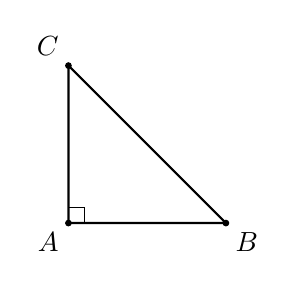
\begin{tikzpicture}[scale=2]
				% Các điểm
				\coordinate (A) at (0,0);
				\coordinate (B) at (1,0);
				\coordinate (C) at (0,1);
				
				% Cạnh tam giác
				\draw[thick] (A) -- (B) -- (C) -- cycle;
				
				% Vẽ các vectơ cần thiết (nhấn mạnh)
				\draw[ black] (B) -- (C);
				\draw[ black] (B) -- (A) ;
				\draw[black] (A) -- (C);
				
				% Ghi nhãn các điểm
				\filldraw[black] (A) circle (0.5pt) node[below left] {$A$};
				\filldraw[black] (B) circle (0.5pt) node[below right] {$B$};
				\filldraw[black] (C) circle (0.5pt) node[above left] {$C$};
				
				% Ký hiệu vuông góc
				\draw (A) -- ++(0,0.1) -- ++(0.1,0)-- ++(0,-0.1);
			\end{tikzpicture}
		\end{center}
	}
\end{ex}
\begin{ex}%[0H5N4-3]%[Dự án đề cương 3 Khối NH24-25-Dot 1-Nguyễn Hoài Nam]
	Cho tam giác đều $ABC$. Phát biểu nào sau đây đúng?
	\choice
	{$\overrightarrow{AB} - \overrightarrow{BC} = \overrightarrow{0}$}
	{\True $\left|\overrightarrow{AB}\right| = \left|\overrightarrow{AC}\right|$}
	{$\overrightarrow{AB} = \overrightarrow{AC}$}
	{$\overrightarrow{AB} + \overrightarrow{BC} = \overrightarrow{CA}$}
	
	\loigiai{
		Vì tam giác $ABC$ là tam giác đều nên các cạnh có độ dài bằng nhau.\\
		Do đó, $\left|\overrightarrow{AB}\right| = \left|\overrightarrow{AC}\right|$.}
\end{ex}
\begin{ex}%[0H5N4-1]%[Dự án đề cương 3 Khối NH24-25-Dot 1-Nguyễn Hoài Nam]
	Cho tam giác $ABC$ vuông ở $A$ có góc $\widehat{ABC} = 60^\circ$. Số đo góc giữa hai vectơ $\overrightarrow{AC}$ và $\overrightarrow{CB}$ bằng
	\choice
	{$30^\circ$}
	{$60^\circ$}
	{ $120^\circ$}
	{\True  $150^\circ$}
	
	\loigiai{
		Ta có $\triangle ABC$ vuông tại $A$, $\widehat{ABC} = 60^\circ$ nên $\widehat{CAB} = 30^\circ$.\\
		Dựng véc- tơ $\overrightarrow{CH}=\overrightarrow{AC}\Rightarrow \left( \overrightarrow{AC}, \overrightarrow{CB} \right)= \left( \overrightarrow{CE}, \overrightarrow{CB} \right)=\widehat{BCE} = 180^\circ - \widehat{C} = 180^\circ - 30^\circ = 150^\circ.$
		
		\begin{center}
			\begin{tikzpicture}[scale=2]
				% Định nghĩa các điểm
				\coordinate (A) at (0,0);
				\coordinate (C) at (2,0);
				\coordinate (B) at (0,1.15);
				\coordinate (E) at (4,0);
				% Tam giác
				\draw (A) -- (B) -- (C) -- cycle
				 (A) -- (C) -- (E) 
				(C) -- (B) ;
				
				% Ghi chú điểm
				\filldraw (A) circle (0.5pt) node[below left] {$A$};
				\filldraw (B) circle (0.5pt) node[above left] {$B$};
				\filldraw (C) circle (0.5pt) node[below right] {$C$};
				\filldraw (E) circle (0.5pt) node[below left] {$E$};
				% Góc vuông
				\draw (A) -- ++(0,0.1) -- ++(0.1,0)-- ++(0,-0.1);
				
				% Góc tại C
				%	\pic["$150^\circ$", draw=black, angle eccentricity=1.3, angle radius=12] {angle=B--C--A};
				
			\end{tikzpicture}
		\end{center}
	}
\end{ex}

\begin{ex}%[0H5N4-1]%[Dự án đề cương 3 Khối NH24-25-Dot 1-Nguyễn Hoài Nam]
	Cho hình vuông $ABCD$ cạnh $a$. Tính $P=\overrightarrow{AC}\cdot \left(\overrightarrow{CD}+\overrightarrow{CA}\right)$.
	\choice
	{$P=-1$}
	{$P=3a^2$}
	{\True $P=-3a^2$}
	{$P=2a^2$}
	\loigiai{
		Ta có $\overrightarrow{AC}\cdot\left(\overrightarrow{CD}+\overrightarrow{CA}\right)= \overrightarrow{AC} \cdot \overrightarrow{CD}-AC^2=AC\cdot CD \cdot \cos 135^\circ -AC^2= -3a^2$.
	}
\end{ex}

\begin{ex}%[0H5N4-1]%[Dự án đề cương 3 Khối NH24-25-Dot 1-Nguyễn Hoài Nam]
	Cho $\overrightarrow{a}$ và $\overrightarrow{b}$ là hai véc-tơ cùng hướng và đều khác véc-tơ $\overrightarrow{0}$. Mệnh đề nào sau đây đúng?
	\choice
	{\True $\overrightarrow{a}\cdot\overrightarrow{b}=\left|\overrightarrow{a}\right|\cdot\left|\overrightarrow{b}\right|$}
	{$\overrightarrow{a}\cdot\overrightarrow{b}=0$}
	{$\overrightarrow{a}\cdot\overrightarrow{b}=-1$}
	{$\overrightarrow{a}\cdot\overrightarrow{b}=-\left|\overrightarrow{a}\right|\cdot\left|\overrightarrow{b}\right|$}
	\loigiai{
		Vì $\overrightarrow{a}$ và $\overrightarrow{b}$ cùng hướng nên $\left(\overrightarrow{a},\overrightarrow{b}\right)=0^\circ$. Do đó $\overrightarrow{a}\cdot\overrightarrow{b}=\left|\overrightarrow{a}\right|\cdot\left|\overrightarrow{b}\right|\cdot \cos 0^\circ=\left|\overrightarrow{a}\right|\cdot\left|\overrightarrow{b}\right|$.
	}
\end{ex}
\begin{ex}%[0H5H4-1]%[Dự án đề cương 3 Khối NH24-25-Dot 1-Nguyễn Hoài Nam]
	Cho hình vuông $ABCD$ có cạnh $a$. Tính $\overrightarrow{AB} \cdot \overrightarrow{AD}$.
	\choice
	{\True $0$}
	{$a$}
	{$\dfrac{a^2}{2}$}
	{$a^2$}
	
	\loigiai{
		\begin{center}
			\begin{tikzpicture}[scale=1, >=stealth]
				% Định nghĩa các điểm
				\coordinate (A) at (0,0);
				\coordinate (B) at (4,0);
				\coordinate (C) at (4,4);
				\coordinate (D) at (0,4);
				
				% Vẽ hình vuông
				\draw (A) -- (B) -- (C) -- (D) -- cycle;
				
				% Vẽ các vectơ
				\draw[->, black] (A) -- (B)  ;
				\draw[->, black] (C) -- (A) ;
				
				% Gán nhãn
				\node[below left] at (A) {$A$};
				\node[below right] at (B) {$B$};
				\node[above right] at (C) {$C$};
				\node[above left] at (D) {$D$};
			\end{tikzpicture}
		\end{center}
		Ta có $AB \perp AD$ nên $\overrightarrow{AB} \cdot \overrightarrow{AD}=0$.
	}
\end{ex}
\begin{ex}%[0H5H4-1]%[Dự án đề cương 3 Khối NH24-25-Dot 1-Nguyễn Hoài Nam]
	Cho hình chữ nhật $ABCD$ có $AB = 4a$ và $AD = 3a$. Độ dài của véc-tơ $\overrightarrow{BA} + \overrightarrow{DA}$ bằng
	\choice
	{\True  $5a$}
	{$6a$}
	{$2a\sqrt{3}$}
	{$7a$}
	
	\loigiai{
		Ta có $\overrightarrow{BA} + \overrightarrow{DA}=\overrightarrow{BA} + \overrightarrow{CB}=\overrightarrow{CA}\Rightarrow \left|\overrightarrow{BA} + \overrightarrow{DA}\right|=\left|\overrightarrow{CA}\right|=CA=\sqrt{AB^2+AD^2}=5a$.
		
	}
\end{ex}
\begin{ex}%[0H5H4-1]%[Dự án đề cương 3 Khối NH24-25-Dot 1-Nguyễn Hoài Nam]
	[\textit{Trích đề thi HKI - Trường THPT Chu Văn An, Hà Nội - Năm học 2022-2023}]
	Cho tam giác đều $ABC$ cạnh bằng $2a$. Khi đó $\left|\overrightarrow{AB} + \overrightarrow{AC}\right|$ bằng
	\choice
	{$a$}
	{\True $2\sqrt{3}a$}
	{$\dfrac{\sqrt{3}a}{2}$}
	{$2a$}
	\loigiai{
		\begin{center}
			\begin{tikzpicture}[scale=1, thick]
				% Định nghĩa các điểm
				\coordinate (B) at (0,0);
				\coordinate (C) at (4,0);
				\coordinate (A) at (2,3.5);
				\coordinate (I) at ($(B)!0.5!(C)$); % trung điểm BC
				%		\coordinate (G) at ($(A)!2/3!(I)$); % trọng tâm: chia trung tuyến AM theo tỉ lệ 2:1
				
				% Vẽ tam giác
				\draw (A) -- (B) -- (C) -- cycle;
				
				% Vẽ trung tuyến
				\draw (A) -- (I);
				
				% Gán nhãn các điểm
				\node[above] at (A) {$A$};
				\node[below left] at (B) {$B$};
				\node[below right] at (C) {$C$};
				\node[below] at (I) {$I$};
				%	\node[right] at (G) {$G$};
				
				% Vẽ điểm
				\fill (A) circle (1pt);
				\fill (B) circle (1pt);
				\fill (C) circle (1pt);
				\fill (I) circle (1pt);
				%	\fill (G) circle (1pt);
			\end{tikzpicture}
		\end{center}
		Gọi $I$ là trung điểm của $BC\Rightarrow \left|\overrightarrow{AB} + \overrightarrow{AC}\right|=2\left|\overrightarrow{AI}\right|=2\cdot\dfrac{2a\sqrt{3}}{2}=2a\sqrt{3} $.
	}
\end{ex}
\begin{ex}%[0H5H4-1]%[Dự án đề cương 3 Khối NH24-25-Dot 1-Nguyễn Hoài Nam]
	[\textit{Trích đề thi HKI - Trường THPT Trưng Vương, TPHCM - Năm học 2024-2025}]
	Cho tam giác $ABC$ đều có cạnh $AB = 5$, $H$ là trung điểm của $BC$. Tính $\left|\overrightarrow{CA} - \overrightarrow{HC}\right|$.
	\choice
	{\True $\dfrac{5\sqrt{7}}{2}$}
	{$\dfrac{5\sqrt{3}}{2}$}
	{$\dfrac{5\sqrt{7}}{4}$}
	{$5$}
	\loigiai{
		\begin{center}
			\begin{tikzpicture}[scale=1]
				% Tọa độ các điểm
				\coordinate (B) at (0,0);
				\coordinate (C) at (5,0);
				\coordinate (A) at (2.5,4.33); % chiều cao tam giác đều cạnh 5 là 5*sqrt(3)/2 ≈ 4.33
				\coordinate (H) at ($(B)!0.5!(C)$); % Trung điểm BC
				\coordinate (I) at ($(A)!0.5!(H)$); % Trung điểm BC
				% Các cạnh tam giác
				\draw[thick] (A) -- (B) -- (C) -- cycle;
				
				% Vẽ vector CA
				\draw[->, thick, black] (C) -- (A) -- (H) (C) -- (I);
				
				% Vẽ vector HC
				\draw[->, thick, black] (H) -- (C) ;
				
				% Các điểm
				\filldraw[black] (A) circle (1pt) node[above] {$A$};
				\filldraw[black] (B) circle (1pt) node[below left] {$B$};
				\filldraw[black] (C) circle (1pt) node[below right] {$C$};
				\filldraw[black] (H) circle (1pt) node[below] {$H$};
				\filldraw[black] (I) circle (1pt) node[below left] {$I$};
				% Ghi chú cạnh
				%\node at (2.5,-0.4) {$5$};
			\end{tikzpicture}
		\end{center}
		Vì tam giác $ABC$ đều nên các cạnh bằng nhau: $AB = BC = CA = 5$.
		
		Gọi $H$ là trung điểm của $BC$, ta có
		\[
		BH = HC = \dfrac{5}{2},\ AH=\dfrac{5\sqrt{3}}{2}.
		\] 
		Ta có $\left|\overrightarrow{CA} - \overrightarrow{HC}\right|=2\cdot\left|\overrightarrow{CA} + \overrightarrow{CH}\right|=2\left|\overrightarrow{CI}\right|=\sqrt{CH^2+HI^2}=2\cdot\sqrt{\left(\dfrac{5}{2}\right)^2+\left(\dfrac{5\sqrt{3}}{4}\right)^2}=\dfrac{5\sqrt{7}}{2}$.
	}
\end{ex}
\begin{ex}%[0H5H4-1]%[Dự án đề cương 3 Khối NH24-25-Dot 1-Nguyễn Hoài Nam]
	[\textit{Trích đề thi HKI - Trường THPT chuyên Bình Long, Bình Phước - Năm học 2023-2024}]
	Cho hai véc-tơ $\overrightarrow{a}$ và $\overrightarrow{b}$ thỏa mãn $\left|\overrightarrow{a}\right|=3$, $\left|\overrightarrow{b}\right|=2$ và $\overrightarrow{a}\cdot\overrightarrow{b}=-3$. Khi đó góc $\alpha$ giữa hai véc-tơ $\overrightarrow{a}$ và $\overrightarrow{b}$ bằng 
	\choice
	{$30^\circ$}
	{$45^\circ$}
	{$60^\circ$}
	{\True $120^\circ$}
	\loigiai{
		Ta có $\overrightarrow{a}\cdot\overrightarrow{b}=\left|\overrightarrow{a}\right|\cdot\left|\overrightarrow{b}\right|\cdot \cos\alpha\Leftrightarrow -3=3\cdot 2\cdot\cos\alpha\Leftrightarrow\cos\alpha=-\dfrac{1}{2}\Leftrightarrow\alpha=120^\circ$.
	}
\end{ex}



\Closesolutionfile{ans}

\ind{PHẦN II.} \inden{Câu trắc nghiệm đúng sai. Trong mỗi ý a), b), c), d) ở mỗi câu, học sinh chọn đúng hoặc sai.}\\
\setcounter{ex}{0}
\Opensolutionfile{ans}[ans/0H5-Bai4-DS]

\begin{ex}%[0H5H4-1][0H5H4-3][0H5V4-4]%[Dự án đề cương 3 Khối NH24-25-Dot 1-Nguyễn Hoài Nam]
	[\textit{Trích đề thi HKI - Trường THPT Phan Châu Trinh, Đà Nẵng - Năm học 2023-2024}]
	Cho tam giác $ABC$ có $AB = 4\sqrt{2}$, $AC = 6$, $\widehat{BAC} = 45^\circ$. Gọi $D$ là trung điểm của đoạn thẳng $BC$. Điểm $E$ thỏa mãn $\overrightarrow{AE} = k\overrightarrow{AC}$ ($k \in \mathbb{R}$).
	\choiceTF
	{$AB \cdot AC = 20$}
	{\True $\overrightarrow{AD} = \dfrac{1}{2}\overrightarrow{AB} + \dfrac{1}{2}\overrightarrow{AC}$}
	{$BC = 3\sqrt{5}$}
	{\True $AD \perp BE$ khi $k = \dfrac{14}{15}$}
	\loigiai{
		\begin{center}
				\begin{tikzpicture}[scale=1, font=\footnotesize, line join=round, line cap=round, >=stealth]
				\path 
				(1,2) coordinate (A)
				(0,0) coordinate (B)
				(4,0) coordinate (C)
				(2,0) coordinate (D)
				(2.5,1) coordinate (E)
				
				;
				
				
				\draw (A)--(B)--(C)--(A) (D)--(A) (B)--(E) ;
				\foreach \x/\g in {A/90,B/180,C/0,D/-90,E/45}
				\fill[black] 	(\x) circle (1pt)
				($(\g:3mm)+(\x)$) node {$\x$};
			\end{tikzpicture}
		\end{center}
		\begin{enumerate} 
			\item Ta có
			$\overrightarrow{AB} \cdot \overrightarrow{AC} = AB \cdot AC \cdot \cos A = 4\sqrt{2} \cdot 6 \cdot \cos 45^\circ = 24.$
			
			\item  Ta có
			$\overrightarrow{BC} = \overrightarrow{AC} - \overrightarrow{AB}; \quad \overrightarrow{AD} = \dfrac{1}{2} \overrightarrow{AB} + \dfrac{1}{2} \overrightarrow{AC}.$\\
			Khi đó
			\allowdisplaybreaks
			\begin{eqnarray*}
					BC^2 &=& \left| \overrightarrow{AC} - \overrightarrow{AB} \right|^2 \\
					&=& AC^2 - 2\overrightarrow{AC} \cdot \overrightarrow{AB} + AB^2 \\
					&=& 6^2 - 2 \cdot 24 + \left(4\sqrt{2}\right)^2 = 36 - 48 + 32 = 20 \\
					\Rightarrow BC& =& 2\sqrt{5}.
			\end{eqnarray*}
			Mặt khác
			\allowdisplaybreaks{\begin{eqnarray*}
					AD^2 &=& \left( \dfrac{1}{2} \overrightarrow{AB} + \dfrac{1}{2} \overrightarrow{AC} \right)^2 \\
					&=& \dfrac{1}{4} \left( \overrightarrow{AB} + \overrightarrow{AC} \right)^2 \\
					&=& \dfrac{1}{4} \left( AB^2 + 2\overrightarrow{AB} \cdot \overrightarrow{AC} + AC^2 \right)\\
					&=&\dfrac{1}{4}\left[\left(4\sqrt{2}\right)^2+2\cdot 24+6^2\right]=29.
			\end{eqnarray*}}
			Suy ra $AD=\sqrt{29}$. 
			\item  Ta có
			$
			\overrightarrow{BE} = \overrightarrow{AE} - \overrightarrow{AB} = k\overrightarrow{AC} - \overrightarrow{AB}.
			$
			Từ đó ta có
			\allowdisplaybreaks{\begin{eqnarray*}
					\overrightarrow{AD} \cdot \overrightarrow{BE} 
					&=& \dfrac{1}{2} \left( \overrightarrow{AB} + \overrightarrow{AC} \right) \cdot \left( k\overrightarrow{AC} - \overrightarrow{AB} \right) \\
					&=& \dfrac{1}{2} \left( k\overrightarrow{AB} \cdot \overrightarrow{AC} + kAC^2 - AB^2 - \overrightarrow{AB} \cdot \overrightarrow{AC} \right) \\
					&=& \dfrac{1}{2} \left( 24k + 36k - \left(4\sqrt{2}\right)^2 - 24 \right) \\
					&=& \dfrac{1}{2} \left( 60k - 40 \right) = 30k - 20.
			\end{eqnarray*}}
			\item Khi đó $AD \perp BE \Leftrightarrow \overrightarrow{AD} \cdot \overrightarrow{BE} = 0
			\Leftrightarrow 30k - 28 = 0 \Leftrightarrow k = \dfrac{14}{15}.$
		\end{enumerate} 
	}
\end{ex}
\begin{ex}%[0H5H4-1][0H5H4-3][0H5V4-4]%[Dự án đề cương 3 Khối NH24-25-Dot 1-Nguyễn Hoài Nam]
	[\textit{Trích đề thi HKI - Trường THPT Phước Bình, Bình Phước - Năm học 2024-2025}]
	Cho tam giác $ABC$ có $AB = 2a$, $AC = 3a$, $\widehat{BAC} = 60^\circ$. Gọi $I$ là trung điểm đoạn thẳng $BC$. 
	Điểm $J$ thuộc đoạn $AC$ thỏa mãn $12AJ = 7AC$. 
	\choiceTF
	{$\overrightarrow{AB} \cdot \overrightarrow{AC} = 4a^2$}
	{$\overrightarrow{AI} = \dfrac{3}{2} \overrightarrow{AB} + \dfrac{3}{2} \overrightarrow{AC}$}
	{\True $\overrightarrow{BJ} = -\overrightarrow{AB} + \dfrac{7}{12} \overrightarrow{AC}$}
	{\True $AI \perp BJ$}
	\loigiai{
		\begin{center}
			\begin{tikzpicture}[scale=1, font=\footnotesize, line join=round, line cap=round, >=stealth]
				% Định nghĩa các điểm
				\coordinate (A) at (0,0);
				\coordinate (B) at (2,0);
				\coordinate (C) at (60:3); % AC = 3, góc 60 độ
				\coordinate (I) at ($(B)!0.5!(C)$);
				\coordinate (J) at ($(A)!7/12!(C)$);
				
				% Vẽ tam giác và các đoạn thẳng
				\draw (A) -- (B) -- (C) -- cycle;
				\draw (A) -- (I);
				\draw (B) -- (J);
				
				\foreach \x/\g in {A/180,B/0,C/90,I/0,J/135}
				\fill[black] 	(\x) circle (1pt)
				($(\g:3mm)+(\x)$) node {$\x$};
			\end{tikzpicture}
		\end{center}
		\begin{enumerate}
			\item  Ta có
			$
			\overrightarrow{AB} \cdot \overrightarrow{AC} = AB \cdot AC \cdot \cos \widehat{BAC} = 2a \cdot 3a \cdot \cos 60^\circ = 3a^2.
			$
			
			\item  Do $I$ là trung điểm $BC$ nên
			$
			\overrightarrow{AI} = \dfrac{1}{2} \left( \overrightarrow{AB} + \overrightarrow{AC} \right) = \dfrac{1}{2} \overrightarrow{AB} + \dfrac{1}{2} \overrightarrow{AC}.
			$
			
			\item  Ta có
			$
			\overrightarrow{BJ} = \overrightarrow{BA} + \overrightarrow{AJ} = -\overrightarrow{AB} + \dfrac{7}{12} \overrightarrow{AC}.
			$
			
			\item  
			\begin{align*}
				\overrightarrow{AI} \cdot \overrightarrow{BJ} 
				&= \left( \dfrac{1}{2} \overrightarrow{AB} + \dfrac{1}{2} \overrightarrow{AC} \right) \cdot \left( -\overrightarrow{AB} + \dfrac{7}{12} \overrightarrow{AC} \right) \\
				&= \dfrac{1}{2} \left( -\overrightarrow{AB}^2 + \dfrac{7}{12} \overrightarrow{AB} \cdot \overrightarrow{AC} - \overrightarrow{AC} \cdot \overrightarrow{AB} + \dfrac{7}{12} \overrightarrow{AC}^2 \right) \\
				&= \dfrac{1}{2} \left( -4a^2 + \dfrac{7}{12} \cdot 3a^2 - 3a^2 + \dfrac{7}{12} \cdot 9a^2 \right) \\
				&= \dfrac{1}{2} \left( -4a^2 + \dfrac{7}{4} a^2 - 3a^2 + \dfrac{21}{4} a^2 \right) \\
				&= \dfrac{1}{2} \cdot 0 = 0.
			\end{align*}
			Vậy $AI \perp BJ$.
		\end{enumerate}
	}
\end{ex}
\begin{ex}%[0H5V4-1]%[Dự án đề cương 3 Khối NH24-25-Dot 1-Nguyễn Hoài Nam]
	Cho hai véc-tơ $\overrightarrow{a}$, $\overrightarrow{b}$ thỏa mãn $\left| \overrightarrow{a} \right| = 3$, $\left| \overrightarrow{b} \right| = 4$ và góc $\left( \overrightarrow{a}, \overrightarrow{b} \right) = 60^\circ$. 
	\choiceTF
	{\True $\overrightarrow{a}\cdot \overrightarrow{b} = 6$}
	{$\overrightarrow{a}^2 = 16$}
	{$\left( \overrightarrow{a} + \overrightarrow{b} \right) \left( \overrightarrow{a} - \overrightarrow{b} \right) = 7$}
	{\True $\left| \overrightarrow{a} + \overrightarrow{b} \right| = \sqrt{37}$}
	\loigiai{
		\begin{enumerate}
			\item Ta có $\overrightarrow{a}\cdot \overrightarrow{b} = \left| \overrightarrow{a} \right| \cdot \left| \overrightarrow{b} \right| \cdot \cos\left( \overrightarrow{a}, \overrightarrow{b} \right)
			= 3\cdot 4 \cdot \cos60^\circ = 6$.
			\item Ta có $\overrightarrow{a}^2 = \left| \overrightarrow{a} \right|^2 = 3^2 = 9$.
			\item Ta có $\left( \overrightarrow{a} + \overrightarrow{b} \right) \left( \overrightarrow{a} - \overrightarrow{b} \right) = \overrightarrow{a}^2 - \overrightarrow{b}^2 = \left| \overrightarrow{a} \right|^2 - \left| \overrightarrow{b} \right|^2 = 3^2 - 4^2 = -7$.
			\item Ta có $\left| \overrightarrow{a} + \overrightarrow{b} \right|^2 = \left( \overrightarrow{a} + \overrightarrow{b} \right)^2 = \overrightarrow{a}^2 + 2\overrightarrow{a}\cdot \overrightarrow{b} + \overrightarrow{b}^2 = 3^2 + 2\cdot 6 + 4^2 = 37$ $\Rightarrow \left| \overrightarrow{a} + \overrightarrow{b} \right| = \sqrt{37}$.
		\end{enumerate}		
	}
\end{ex}


\begin{ex}%[0H5V4-4]%[Dự án đề cương 3 Khối NH24-25-Dot 1-Nguyễn Hoài Nam] 
	Cho hình vuông $ABCD$ có cạnh bằng $6$. Gọi $M$, $N$ lần lượt là những điểm thuộc đoạn thẳng $BC$, $CD$ thỏa mãn $BM=\dfrac{1}{3}BC$ và $CN=\dfrac{1}{3}CD$.
	\choiceTF
	{\True $\overrightarrow{BM}\cdot \overrightarrow{CN} = 0$}
	{$\overrightarrow{BM}\cdot \overrightarrow{BC} = 18$}
	{\True Góc giữa $\overrightarrow{AB}$ và $\overrightarrow{CN}$ bằng $180^\circ$}
	{\True $AM\perp BN$}
	\loigiai{
		\begin{center}
			\begin{tikzpicture}[scale=0.8, font=\footnotesize, line join=round, line cap=round, >=stealth]
				\path 
				(0,6) coordinate (A)
				(6,6) coordinate (B)
				(6,0) coordinate (C)
				($(C)+(A)-(B)$) coordinate (D)
				($(B)!0.33!(C)$) coordinate (M)
				($(C)!0.33!(D)$) coordinate (N)
				;
				\draw (A)--(B)--(C)--(D)--cycle (A)--(M) (B)--(N);
				\foreach \x/\g in {A/135,B/45,C/-45,D/-135,M/0,N/-90}
				\fill[black] (\x) circle (1pt) + (\g:3mm) node {$\x$};
			\end{tikzpicture}
		\end{center}
		\begin{enumerate}
			\item  Do $BM\perp CN$ nên $\overrightarrow{BM}\cdot \overrightarrow{CN} = 0$.
			\item  $\overrightarrow{BM}\cdot \overrightarrow{BC} = BM \cdot BC \cdot \cos\left( \overrightarrow{BM},\overrightarrow{BC} \right) = 2\cdot 6 \cdot \cos 0^\circ = 12$.
			\item  Do hai véc-tơ $\overrightarrow{AB}$ và $\overrightarrow{CN}$ ngược hướng nên góc giữa chúng bằng $180^\circ$.
			\item 
			\allowdisplaybreaks
			\begin{eqnarray*}
				\overrightarrow{AM} \cdot \overrightarrow{BN} &=& \left( \overrightarrow{AB} + \overrightarrow{BM} \right) \left( \overrightarrow{BC} + \overrightarrow{CN} \right)\\
				&=& \overrightarrow{AB}\cdot \overrightarrow{BC} + \overrightarrow{AB}\cdot \overrightarrow{CN} + \overrightarrow{BM}\cdot \overrightarrow{BC} + \overrightarrow{BM}\cdot \overrightarrow{CN}\\
				&=& 0 + AB\cdot CN\cdot \cos\left( \overrightarrow{AB},\overrightarrow{CN} \right) + BM\cdot BC\cdot \cos \left(\overrightarrow{BM}, \overrightarrow{BC} \right) + 0\\
				&=& 6\cdot 2\cdot \cos180^\circ + 2\cdot 6\cdot \cos0^\circ \\
				&=& 0.
			\end{eqnarray*}
			Suy ra $\overrightarrow{AM} \perp \overrightarrow{BN}$, nên $AM\perp BN$.
		\end{enumerate}
	}
\end{ex}


\begin{ex}%[0H5V4-1]%[Dự án đề cương 3 Khối NH24-25-Dot 1-Nguyễn Hoài Nam]
	Cho hình chữ nhật $ABCD$ tâm $O$ có $AB=4$, $BC=3$
	\choiceTF
	{\True $AO=\dfrac{5}{2}$}
	{$\overrightarrow{AC}\cdot \overrightarrow{AB} = 9$}
	{\True $\overrightarrow{AC}\cdot \overrightarrow{BD}=-7$}
	{$\cos\left( \overrightarrow{AO}, \overrightarrow{OD} \right) = -\dfrac{14}{25}$}
	\loigiai{
		\begin{center}
			\begin{tikzpicture}[scale=0.8, font=\footnotesize, line join=round, line cap=round, >=stealth]
				\path 
				(0,3) coordinate (A)
				(4,3) coordinate (B)
				(4,0) coordinate (C)
				($(C)+(A)-(B)$) coordinate (D)
				($(B)!0.5!(D)$) coordinate (O)
				;
				\draw (A)--(B)--(C)--(D)--cycle (A)--(C) (B)--(D);
				\foreach \x/\g in {A/135,B/45,C/-45,D/-135,O/-90}
				\fill[black] (\x) circle (1pt) + (\g:3mm) node {$\x$};
			\end{tikzpicture}
		\end{center}
		\begin{enumerate}
			\item Ta có $AO = \dfrac{1}{2}AC = \dfrac{1}{2}\sqrt{AB^2 + BC^2} = \dfrac{1}{2}\sqrt{4^2+3^2} = \dfrac{5}{2}$.
			\item  
			\allowdisplaybreaks
			\begin{eqnarray*}
				\overrightarrow{AC}\cdot \overrightarrow{AB} &=& \left( \overrightarrow{AB} + \overrightarrow{BC} \right)\cdot \overrightarrow{AB}\\
				&=& \overrightarrow{AB}^2 + \overrightarrow{BC}\cdot \overrightarrow{AB} \\
				&=& 4^2 + 0 \text{ (do } BC\perp AB)\\
				&=& 16.
			\end{eqnarray*}
			\item 
			\allowdisplaybreaks
			\begin{eqnarray*}
				\overrightarrow{AC}\cdot \overrightarrow{BD} &=& \left( \overrightarrow{AB} + \overrightarrow{BC} \right) \left( \overrightarrow{BA} + \overrightarrow{AD} \right)\\
				&=& \overrightarrow{AB}\cdot \overrightarrow{BA} + \overrightarrow{AB}\cdot \overrightarrow{AD} + \overrightarrow{BC}\cdot \overrightarrow{BA} + \overrightarrow{BC}\cdot \overrightarrow{AD}\\
				&=& -\overrightarrow{AB}^2 + 0 + 0 + \overrightarrow{BC}^2\\
				&=& -4^2 + 3^2\\
				&=& -7.
			\end{eqnarray*}
			\item  Ta có $\overrightarrow{AO} \cdot \overrightarrow{OD} = \dfrac{1}{2}\overrightarrow{AC} \cdot \dfrac{1}{2}\overrightarrow{BD} = \dfrac{1}{4}\overrightarrow{AC}\cdot \overrightarrow{BD} = -\dfrac{7}{4}$.\\
			Suy ra 
			$$\cos\left( \overrightarrow{AO}, \overrightarrow{OD} \right) 
			= \dfrac{\overrightarrow{AO}\cdot \overrightarrow{OD}}{AO\cdot OD}\\
			= \dfrac{-\dfrac{7}{4}}{\dfrac{5}{2}\cdot \dfrac{5}{2}}\\
			= -\dfrac{7}{25}.$$
		\end{enumerate}
	}
\end{ex}
\Closesolutionfile{ans}


\ind{PHẦN III.} \inden{Câu trắc nghiệm trả lời ngắn.}\\
\setcounter{ex}{0}
\Opensolutionfile{ans}[ans/0H5-Bai4-TLN]

\begin{ex}%[0H5H2-1]%[Dự án đề cương 3 Khối NH24-25-Dot 1-Nguyễn Hoài Nam]
	[\textit{Trích đề thi HKI - Trường THPT Ngô Quyền, Quảng Bình - Năm học 2023-2024}]
	Cho hai véc-tơ $\overrightarrow{a}$ và $\overrightarrow{b}$ khác véc-tơ $\overrightarrow{0}$. Khi $\overrightarrow{a}\cdot\overrightarrow{b}=-\left|\overrightarrow{a}\right|\cdot\left|\overrightarrow{b}\right|$ thì góc $\alpha$ giữa hai véc-tơ $\overrightarrow{a}$ và $\overrightarrow{b}$ bằng bao nhiêu độ?
	\shortans{$180$}
	\loigiai{
		Ta có $\overrightarrow{a}\cdot\overrightarrow{b}=-\left|\overrightarrow{a}\right|\cdot\left|\overrightarrow{b}\right|\Leftrightarrow \cos\alpha=-1\Leftrightarrow \alpha=180^\circ$.
	}
\end{ex}
\begin{ex}%[0H5V4-3]%[Dự án đề cương 3 Khối NH24-25-Dot 1-Nguyễn Hoài Nam]
	[\textit{Trích đề thi HKI - Trường THPT Lê Lợi, Quảng Trị - Năm học 2024-2025}]
	Cho hai véc-tơ $ \overrightarrow{a} $ và $ \overrightarrow{b} $ có độ dài bằng $ 1 $ và thỏa mãn điều kiện $ \big | 2\overrightarrow{a}-3\overrightarrow{b} \big |=\sqrt{7} $. Tính $ \cos \left (\overrightarrow{a},\overrightarrow{b}\right ) $.
	\shortans{$-1$}
	\loigiai{
		\[ \big | 2\overrightarrow{a}-3\overrightarrow{b} \big |=\sqrt{7}\Leftrightarrow \left (2\overrightarrow{a}-3\overrightarrow{b}\right )^2=7 \Leftrightarrow 4\big|\overrightarrow{a}\big|^2-6\overrightarrow{a}\cdot \overrightarrow{b}+9\big|\overrightarrow{b}\big|^2=7\Leftrightarrow \overrightarrow{a}\cdot \overrightarrow{b}=-1. \]
		Do đó $\cos \left (\overrightarrow{a},\overrightarrow{b}\right )=\dfrac{\overrightarrow{a}\cdot \overrightarrow{b}}{\big|\overrightarrow{a}\big|\cdot \big|\overrightarrow{b}\big|}=-1$.
	}
\end{ex}
\begin{ex}%[0H5V2-1]%[Dự án đề cương 3 Khối NH24-25-Dot 1-Nguyễn Hoài Nam]
	[\textit{Trích đề thi HKI - Trường THPT Hai Bà Trưng, Thừa Thiên Huế - Năm học 2024-2025}]
	Cho hình vuông $ABCD$ cạnh $2$.  Gọi $E$ là điểm đối xứng của $D$ qua $C$. Tính $\overrightarrow{AE}\cdot\overrightarrow{AB}$. 
	\shortans{$8$}
	\loigiai{
		Ta có $\overrightarrow{AE}\cdot\overrightarrow{AB}=\left(\overrightarrow{AB}+\overrightarrow{AC}\right)\cdot \overrightarrow{AB}=\overrightarrow{AB^2}+\overrightarrow{AB}\cdot \overrightarrow{AC}=2^2+2\cdot 2\sqrt{2}\cdot \cos 45^{\circ}=8$.
	}
\end{ex}
\begin{ex}%[0H5V2-1]%[Dự án đề cương 3 Khối NH24-25-Dot 1-Nguyễn Hoài Nam]
	[\textit{Trích đề thi HKI - Trường THPT Hàm Thuận Nam, Bình Thuận - Năm học 2023-2024}]
	Cho tam giác $ABC$ đều cạnh bằng $1$. Tính $\overrightarrow{AB} \cdot \overrightarrow{BC}$.
	\shortans{$0{,}5$}
	\loigiai{
		\begin{center}
			\begin{tikzpicture}[line join=round, line cap=round]
				\def\canh{5}
				\coordinate (B) at (0,0);
				\coordinate (C) at (\canh,0);
				\coordinate (A) at ($(B) + (60:\canh)$);
				\coordinate (D) at ($(A) + (\canh,0)$);
				\path (A)--(B) node[midway,sloped,scale=0.5]{$|$};
				\path (A)--(C) node[midway,sloped,scale=0.5]{$|$};
				\path (B)--(C) node[midway,sloped,scale=0.5]{$|$};
				\coordinate (Tempta) at ($(A)!0.5!(B)$);
				\coordinate (Temptb) at ($(A)!0.5!(C)$);
				\coordinate (Temptc) at ($(Tempta)!1cm!90:(A)$);
				\coordinate (Temptd) at ($(Temptb)!1cm!90:(A)$);
				
				\draw(A)--(B)--(C)--cycle (A)--(D);
				\foreach \i/\g in {A/90,B/-90,C/-90,D/90}{\draw[fill=black](\i) circle (1.5pt) ($(\i)+(\g:3mm)$) node[scale=1]{$\i$};}
			\end{tikzpicture}
		\end{center}		
		Gọi $D$ là điểm sao cho $\overrightarrow{AD}=\overrightarrow{BC}$.\\
		Vì $AD\parallel BC$ nên $\widehat{DAC}=\widehat{ACB}=60^{\circ}$.\\
		Suy ra $\widehat{BAD}=\widehat{DAC}+\widehat{BAC}=60^{\circ}+60^{\circ}=120^{\circ}$.\\
		$\overrightarrow{AB} \cdot \overrightarrow{BC}=\overrightarrow{AB} \cdot \overrightarrow{AD}=\left|\overrightarrow{AB}\right|\cdot\left|\overrightarrow{AD}\right|\cos\left(\overrightarrow{AB},\overrightarrow{AD}\right)=\left|\overrightarrow{AB}\right|\cdot\left|\overrightarrow{AD}\right|\cos\widehat{BAD}=1\cdot 1 \cdot \cos 120^{\circ}=-0{,}5$.
	}
\end{ex}
\begin{ex}%[0H5V2-1]%[Dự án đề cương 3 Khối NH24-25-Dot 1-Nguyễn Hoài Nam]
	Cho hình thang $ABCD$ có đáy lớn $BC=3a$, đáy nhỏ $AD=a$, đường cao $AB=2a$. Gọi $I$ là trung điểm $CD$. Tính góc giữa $AI$ và $BD$ (đơn vị độ).
	\shortans{$90$}
	\loigiai{
		\begin{center}
			\begin{tikzpicture}[>=stealth,line join=round,line cap=round,font=\footnotesize,scale=0.7]
				\path (0,0) coordinate (B)
				(6,0) coordinate (C)
				(2,0) coordinate (H)
				(0,4) coordinate (A)
				(2,4) coordinate (D)
				($(C)!1/2!(D)$)  coordinate (I)
				;
				\draw (A)--(B)--(C)--(D)--cycle (B)--(D)--(H) (I)--(A)--(C);
				\foreach \t/\g in {B/180,C/0,D/0,A/180,H/-90,I/0}{
					\draw[fill=black] (\t) circle (1pt) node[shift={(\g:7pt)},font=\scriptsize]{$ \t $};
				}
			\end{tikzpicture}
		\end{center}
		Vẽ đường cao $DH$ ta có\\
		Ta có\\
		$\overrightarrow{BC}\cdot \overrightarrow{BD}
		= BC\cdot BD\cdot \cos \widehat{DBC}
		= BD\cdot BC\cdot \dfrac{BH}{BD}
		= 3a\cdot a\sqrt{5}\cdot\dfrac{a}{a\sqrt{5}}
		= 3a^2$.\\
		Ta có \\
		$\overrightarrow{AC}\cdot \overrightarrow{BD}= \left(\overrightarrow{AB}+\overrightarrow{BC}\right)\cdot \overrightarrow{BD}= \overrightarrow{AB}\cdot \overrightarrow{BD}+\overrightarrow{BC}\cdot \overrightarrow{BD}=  AB\cdot BD\cdot \cos (180^\circ-\widehat{ABD})+3a^2$\\
		$= AB\cdot BD\cdot \dfrac{-AB}{BD}+3a^2= 2a\cdot a\sqrt{5}\left(-\dfrac{2a}{a\sqrt{5}}\right)+3a^2=-a^2$.\\
		Ta có\\
		$\overrightarrow{AI}\cdot \overrightarrow{BD}=\dfrac{1}{2}\left(\overrightarrow{AD}+ \overrightarrow{AC}\right)\cdot \overrightarrow{BD}=\dfrac{1}{2}\overrightarrow{AD}\cdot \overrightarrow{BD}+\dfrac{1}{2}\overrightarrow{AC}\cdot \overrightarrow{BD}=\dfrac{1}{2}\cdot a \cdot a\sqrt{5}\cdot  \dfrac{a}{a\sqrt{5}}+\dfrac{1}{2}(-a^2)=0$.\\
		Vậy góc tạo bởi $AI$ và $BD$ là $90^\circ$.
		
	}
\end{ex}
\Closesolutionfile{ans}


\ind{PHẦN IV.} \inden{Tự luận.}\\
\setcounter{ex}{0}
\begin{ex}%[0H5H4-2]%[Dự án đề cương 3 Khối NH24-25-Dot 1-Nguyễn Hoài Nam]
	[\textit{Trích đề thi HKI - Trường THPT Bình Giang, Hải Dương - Năm học 2023-2024}] 
	Tính $\left(\overrightarrow{a},\overrightarrow{b}\right)$ biết rằng $\left|\overrightarrow{a}\right|=3$, $\left|\overrightarrow{b}\right|=4$ và $\overrightarrow{a}\cdot\overrightarrow{b}=-6\sqrt{3}$.
	\loigiai{
		Ta có  $\cos \left(\overrightarrow{a},\overrightarrow{b}\right)=\dfrac{\overrightarrow{a}\cdot\overrightarrow{b}}{\left|\overrightarrow{a}\right|\cdot\left|\overrightarrow{b}\right|}=\dfrac{-6\sqrt{3}}{3\cdot 4}=\dfrac{-\sqrt{3}}{2}$. \\
		Do đó, $\left(\overrightarrow{a},\overrightarrow{b}\right)=150^\circ$.
	}
\end{ex} 

\begin{ex}%[0H5H4-2]%[Dự án đề cương 3 Khối NH24-25-Dot 1-Nguyễn Hoài Nam]
	[\textit{Trích đề thi HKI - Trường THPT Thanh Bình, Cà Mau - Năm học 2024-2025}] 
	Cho hình thoi $ABCD$. Chứng minh rằng
	$$
	\overrightarrow{AB}\cdot(\overrightarrow{BC}+\overrightarrow{BA})+\overrightarrow{AD}\cdot(\overrightarrow{BC}+\overrightarrow{BA})=0.
	$$
	\loigiai{
		Vì $ABCD$ là hình thoi nên $AC\perp BD$. Khi đó, ta có
		$$
		\overrightarrow{AB}\cdot\left(\overrightarrow{BC}+\overrightarrow{BA}\right)+\overrightarrow{AD}\cdot\left(\overrightarrow{BC}+\overrightarrow{BA}\right)
		=\left(\overrightarrow{AB}+\overrightarrow{AD}\right)\cdot\left(\overrightarrow{BC}+\overrightarrow{BA}\right)
		=\overrightarrow{AC}\cdot\overrightarrow{BD}=0.
		$$
	}
\end{ex}

\begin{ex}%[0H5H4-2]%[Dự án đề cương 3 Khối NH24-25-Dot 1-Nguyễn Hoài Nam]
	Cho tam giác $ABC$ vuông tại $A$ có $\widehat{B}=60^\circ$. Tính $\left(\overrightarrow{AB},\overrightarrow{AC}\right)$,$\left(\overrightarrow{CA},\overrightarrow{CB}\right)$, $\left(\overrightarrow{AB},\overrightarrow{BC}\right)$.
	\loigiai{
		\immini{Ta có \\
			$\left(\overrightarrow{AB},\overrightarrow{AC}\right)=\widehat{BAC}=90^\circ$.\\ $\left(\overrightarrow{CA},\overrightarrow{CB}\right)=\widehat{ACB}=30^\circ$. \\
			$\left(\overrightarrow{AB},\overrightarrow{BC}\right)=\left(\overrightarrow{BD},\overrightarrow{BC}\right)=\widehat{DBC}=120^\circ$.
		}{
			\begin{tikzpicture}[>=stealth, line join=round, line cap=round, font=\footnotesize, scale=0.7]
				\coordinate[label=below left:$A$](A) at (0,0);
				\coordinate[label=below right:$B$](B) at (2,0);
				\coordinate[label=above right:$C$](C) at (0,4);
				\coordinate[label=below :$D$](D) at (4,0);
				\draw[dashed] (B)--(D);
				\draw (A)--(B)--(C)--cycle ;
				\path pic[draw,blue,angle radius=4mm] {angle = C--B--A} (B)--($(B)!8mm!($($(B)!8mm!(C)$)!.5!($(B)!8mm!(A)$)$)$)node[scale=1,pos=1]{$60^\circ$};
				\foreach \x/\y/\z in {C/A/B} {
					\path
					($(\y)!5pt!(\z)$) coordinate (1)
					($(\y)!5pt!(\x)$) coordinate (2)
					($(1)+(2)-(\y)$) coordinate (3)
					
					;
					\draw (1)--(3)--(2); }
				\foreach \x in {A,B,C,D}
				\draw[fill=black] (\x) circle (1pt);
			\end{tikzpicture}	 
		}
	}
\end{ex}
\begin{ex}%[0H5H4-2]%[Dự án đề cương 3 Khối NH24-25-Dot 1-Nguyễn Hoài Nam]
	Cho tam giác đều $ABC$. Tính $P=\cos\left(\overrightarrow{AB},\overrightarrow{BC}\right)$.
	\loigiai{
		\immini
		{
			Vẽ $\overrightarrow{BE}=\overrightarrow{AB}$. Khi đó, ta có
			\begin{eqnarray*}
				\left(\overrightarrow{AB},\overrightarrow{BC}\right)&=&\left(\overrightarrow{BE},\overrightarrow{BC}\right) \\
				&=&\widehat{CBE} \\
				&=&180^\circ-\widehat{CBA}=120^\circ.
			\end{eqnarray*}
			Suy ra $\cos\left(\overrightarrow{AB},\overrightarrow{BC}\right)=\cos 120^\circ=-\dfrac{1}{2}$.
		}
		{
			\begin{tikzpicture}[>=stealth,line join=round,line cap=round,font=\footnotesize,scale=1]
				\def\a{3}
				\path
				(0,0) coordinate (A)
				(0:\a) coordinate (B)
				(60:\a) coordinate (C)
				($ (B)+(0:\a) $) coordinate (E);
				\foreach \x/\y in {A/B,B/C,B/E}\draw[->] (\x)--(\y);
				\draw (A)--(C);
				\foreach \x/\g in {A/-90,B/-90,C/90,E/-90}\fill[black] (\x) circle (1pt)+(\g:3mm) node{$ \x $};
			\end{tikzpicture}
		}
	}
\end{ex}
\begin{ex}%[0H5H4-1]%[Dự án đề cương 3 Khối NH24-25-Dot 1-Nguyễn Hoài Nam]
	[\textit{Trích đề thi HKI - Trường THPT Thái Phiên, Hải Phòng - Năm học 2023-2024}]
	Cho tam giác $ABC$ vuông cân tại $B$ và $AB=5$. Tính tích vô hướng $\overrightarrow{AB}\cdot\overrightarrow{AC}$.
	\loigiai{Do tam giác $ABC$ vuông cân tại $B$ nên $\left(\overrightarrow{AB},\overrightarrow{AC}\right)=\widehat{BAC}=45^\circ$ và $AC=5\sqrt{2}$. Suy ra
		$$\overrightarrow{AB}\cdot\overrightarrow{AC}=\left|\overrightarrow{AB}\right|\cdot\left|\overrightarrow{AC}\right|\cdot\cos\left(\overrightarrow{AB},\overrightarrow{AC}\right)=AB\cdot AC\cdot\cos \widehat{BAC}=5\cdot 5\sqrt{2}\cdot \cos 45^\circ=25.$$}
\end{ex}
\begin{ex}%[0H5H4-1]%[Dự án đề cương 3 Khối NH24-25-Dot 1-Nguyễn Hoài Nam]
	Cho hai véc-tơ $\overrightarrow{a}=4\overrightarrow{i}+6\overrightarrow{j}$ và $\overrightarrow{b}=3\overrightarrow{i}-7\overrightarrow{j}$, trong đó $\overrightarrow{i}$ và $\overrightarrow{j}$ là hai véc-tơ có độ dài bằng $1$, vuông góc với nhau. Tính tích vô hướng $\overrightarrow{a}\cdot\overrightarrow{b}$.
	\loigiai{Do $\overrightarrow{i}$, $\overrightarrow{j}$ vuông góc nhau nên $\overrightarrow{i}\cdot\overrightarrow{j}=0$. Khi đó $$\overrightarrow{a}\cdot\overrightarrow{b}=\left(4\overrightarrow{i}+6\overrightarrow{j}\right)\cdot\left(3\overrightarrow{i}-7\overrightarrow{j}\right)=12\overrightarrow{i}^2-42\overrightarrow{j}^2=12-42=-30.$$}
\end{ex}
\begin{ex}%[0H5H4-1]%[Dự án đề cương 3 Khối NH24-25-Dot 1-Nguyễn Hoài Nam]
	Cho hai véc-tơ $\overrightarrow{a}$, $\overrightarrow{b}\neq \overrightarrow{0}$. Tính góc giữa hai véc-tơ $\overrightarrow{a}$, $\overrightarrow{b}$ biết $\overrightarrow{a}\cdot\overrightarrow{b}=\dfrac{1}{2}\left|\overrightarrow{a}\right|\cdot\left|\overrightarrow{b}\right|$.
	\loigiai{Ta có $\cos\left(\overrightarrow{a},\overrightarrow{b}\right)=\dfrac{\overrightarrow{a}\cdot\overrightarrow{b}}{\left|\overrightarrow{a}\right|\cdot\left|\overrightarrow{b}\right|}=\dfrac{\dfrac{1}{2}\left|\overrightarrow{a}\right|\cdot\left|\overrightarrow{b}\right|}{\left|\overrightarrow{a}\right|\cdot\left|\overrightarrow{b}\right|}=\dfrac{1}{2}\Rightarrow \left(\overrightarrow{a},\overrightarrow{b}\right)=60^\circ$.}
\end{ex}
\begin{ex}%[0H5V4-5]%[Dự án đề cương 3 Khối NH24-25-Dot 1-Nguyễn Hoài Nam]
	[\textit{Trích đề thi HKI - Trường THPT chuyên Lương Thế Vinh, Đồng Nai - Năm học 2023-2024}]
	Cho tam giác $ABC$. Tìm tập hợp các điểm $M$ sao cho $\overrightarrow{MA}\cdot\overrightarrow{MB}+\overrightarrow{MA}\cdot\overrightarrow{MC}=0$.
	\loigiai{
		\begin{center}
			\begin{tikzpicture}[scale=1, font=\footnotesize, line join=round, line cap=round, >=stealth]
				\path 
				(0,0) coordinate (B)
				($(B)+(5,0)$) coordinate (C)
				($(B)+(1.5,3.5)$) coordinate (A)
				($(B)!0.5!(C)$) coordinate (I)
				($(A)!0.5!(I)$) coordinate (O)
				($(O)+(4,2.5)$) coordinate (m);
				\path[name path=Om] (O)--(m);
				\draw[name path=O] (O) let\p1=($(O)-(I)$) in circle ({veclen(\x1,\y1)});
				\path[name intersections={of=Om and O}] (intersection-1) coordinate (M);
				\draw (A)--(B)--(C)--cycle (A)--(I) (A)--(M)--(B) (I)--(M)--(C);
				\foreach \i/\j in {B/-135, C/-45, A/90, M/45, I/-90}\draw[fill=black] (\i) circle (1.pt) ++(\j:0.3) node {$\i$};
			\end{tikzpicture}
		\end{center}	
		Gọi $I$ là trung điểm $BC$. Khi đó $$\overrightarrow{MA}\cdot\overrightarrow{MB}+\overrightarrow{MA}\cdot\overrightarrow{MC}=0\Leftrightarrow \overrightarrow{MA}\cdot\left(\overrightarrow{MB}+\overrightarrow{MC}\right)=0\Leftrightarrow\overrightarrow{MA}\cdot 2\overrightarrow{MI}=0\Leftrightarrow \overrightarrow{MA}\cdot\overrightarrow{MI}=0.$$
		Suy ra $M$ thuộc đường tròn đường kính $AI$.\\
		Vậy tập hợp điểm $M$ là đường tròn đường kính $AI$.}
\end{ex}
\begin{ex}%[0H5V4-4]%[Dự án đề cương 3 Khối NH24-25-Dot 1-Nguyễn Hoài Nam]
	Cho hình vuông $ABCD$. Gọi $E$, $F$ lần lượt là trung điểm của $BC$, $CD$. Chứng minh rằng $AE\perp BF$.
	\loigiai{
		\begin{center}
			\begin{tikzpicture}[scale=1, font=\footnotesize, line join=round, line cap=round, >=stealth]
				\path 
				(0,0) coordinate (B)
				($(B)+(3,0)$) coordinate (C)
				($(B)+(0,3)$) coordinate (A)
				($(C)+(0,3)$) coordinate (D)
				($(C)!0.5!(B)$) coordinate (E)
				($(C)!0.5!(D)$) coordinate (F);
				\draw (A)--(B)--(C)--(D)--cycle (A)--(E) (B)--(F);
				\foreach \i/\j in {A/135, B/-135, C/-45, D/45, F/0, E/-90}\draw[fill=black] (\i) circle (1pt) ++(\j:0.3) node {$\i$};
			\end{tikzpicture}
		\end{center}
		Ta có $$\overrightarrow{AE}\cdot\overrightarrow{BF}=\left(\overrightarrow{AB}+\overrightarrow{BE}\right)\cdot\left(\overrightarrow{BC}+\overrightarrow{CF}\right)=\overrightarrow{AB}\cdot\overrightarrow{CF}+\overrightarrow{BE}\cdot\overrightarrow{BC}=-\dfrac{1}{2}AB^2+\dfrac{1}{2}BC^2=0.$$
		Suy ra $AE\perp BF$.}
\end{ex}
\begin{ex}%[0H5V2-2]%[Dự án đề cương 3 Khối NH24-25-Dot 1-Nguyễn Hoài Nam]
	Cho điểm $M$ thay đổi trên đường tròn tâm $O$ bán kính $R$ ngoại tiếp tam giác đều $ABC$ cho trước. Biết rằng $MA^2+2\overrightarrow{MB}\cdot\overrightarrow{MC}=kR^2$. Tìm $k$.
	\loigiai{
		Ta có $\triangle ABC$ đều nên $\widehat{BOC}=2\widehat{BAC}=120^\circ$, $\overrightarrow{OA}+\overrightarrow{OB}+\overrightarrow{OC}=\overrightarrow{0}$. Do đó
		\begin{eqnarray*}
			&& MA^2+2\overrightarrow{MB}\cdot\overrightarrow{MC}\\
			& = & \left(\overrightarrow{MO}+\overrightarrow{OA}\right)^2+2\left(\overrightarrow{MO}+\overrightarrow{OB}\right)\left(\overrightarrow{MO}+\overrightarrow{OC}\right)\\
			& = & 3MO^2+OA^2+2\overrightarrow{OB}\cdot\overrightarrow{OC}+2\overrightarrow{MO}\left(\overrightarrow{OA}+\overrightarrow{OB}+\overrightarrow{OC}\right)\\
			& = & 4R^2+2R^2\cdot\cos{120^\circ}=3R^2.
		\end{eqnarray*}
		Vậy $k=3$.
	}
\end{ex}

